\chapter{Designing Dynamic Mechanisms}
The realistic simulation of highly-dynamic elastic objects is important for a broad range of applications in computer graphics, engineering and computational fabrication. However, whether simulating flipping toys, jumping robots, prosthetics or quickly moving creatures, performing such simulations in the presence of contact, impact and friction is both time consuming and inaccurate. In this paper we present Dynamics-Aware Coarsening (DAC) and the Boundary Balanced Impact (BBI) model  which allow for the accurate simulation of dynamic, elastic objects undergoing both large scale deformation and frictional contact, at rates up to 79 times faster than state-of-the-art methods. DAC and BBI produce simulations that are accurate and fast enough to be used  (for the first time) for the computational design of 3D-printable compliant dynamic mechanisms. Thus we demonstrate the efficacy of DAC and BBI by designing and fabricating mechanisms which flip, throw and jump over and onto obstacles as requested.
\section{Introduction}

We present a pair of new methods to accurately simulate geometric and material nonlinearities subject to frictional contact, large loads and high-speed collisions at rates significantly more than an order-of-magnitude faster than previously available.
Our methods combine efficiency and accuracy to enable design-for-fabrication optimization. They can be used for both fast, realistic animation and engineering analysis. 

Here we look towards a new generation of efficient mechanisms for practical \emph{dynamic} function~\citep{Lipson:2014fa,Rus:2015eq,Reis:2015hb,Reis:2015ey}. In order to extend physics-driven computational design to this domain, however, a bottleneck must be overcome - the physical simulation itself. Simulations must accurately replicate the behavior of elastic materials subject to high-speed, transient dynamics. Modeling these systems combines many of the remaining grand challenges in simulating elastica. Specifically we must accurately resolve nonlinear elasticity, large deformations, stiff materials, high-speed dynamics, rapid loading and unloading, frictional contact, internal friction, high-speed collisions, and rebound. 

State-of-the-art FEM systems currently able to accurately match these effects are exceedingly expensive - runtimes on the order of days are standard to perform a single simulation in many cases~\citep{Belytschko:2013tz}. 
Thus, while generating a single simulation for visualization or animation is already time consuming, the many simulations required during design optimization compound an already prohibitive computational burden.
\subsection{Efficiency with Accuracy}
Let us explore four potential solutions for constructing fast \emph{and} accurate simulation algorithms: (1) higher-order elements, (2) adaptive meshes, (3) reduced models, and (4) numerical coarsening. Can these methods provide the necessary efficiency to enable design-optimization while obtaining the predictive accuracy required to match fabricated results?

\emph{Higher-order elements} offer us the opportunity to replace thin regions of our models with elements that capture higher-order deformation modes. While an attractive strategy, this poses two challenges. 
First, due to changing design parameters, we will need to identify suitable regions on-the-fly in order to perform this replacement. 
Second, coupling swapped-in higher-order elements to other element types introduces overhead. Consider, for example, replacing lower-order hexahedra with plate elements in these regions. We must then ensure continuity of displacements between plate-like portions of the design and thicker, volumetric portions. This, in turn, requires introducing difficult coupling constraints~\cite{Bergou2007,Martin:2010:USE}. Finally, even with such additional efforts, these substitutions may not always improve computational performance as high-order elements contain more DoFs than their low-order counterparts~\cite{Belytschko:2013tz}. 

\begin{figure}
	\centering
	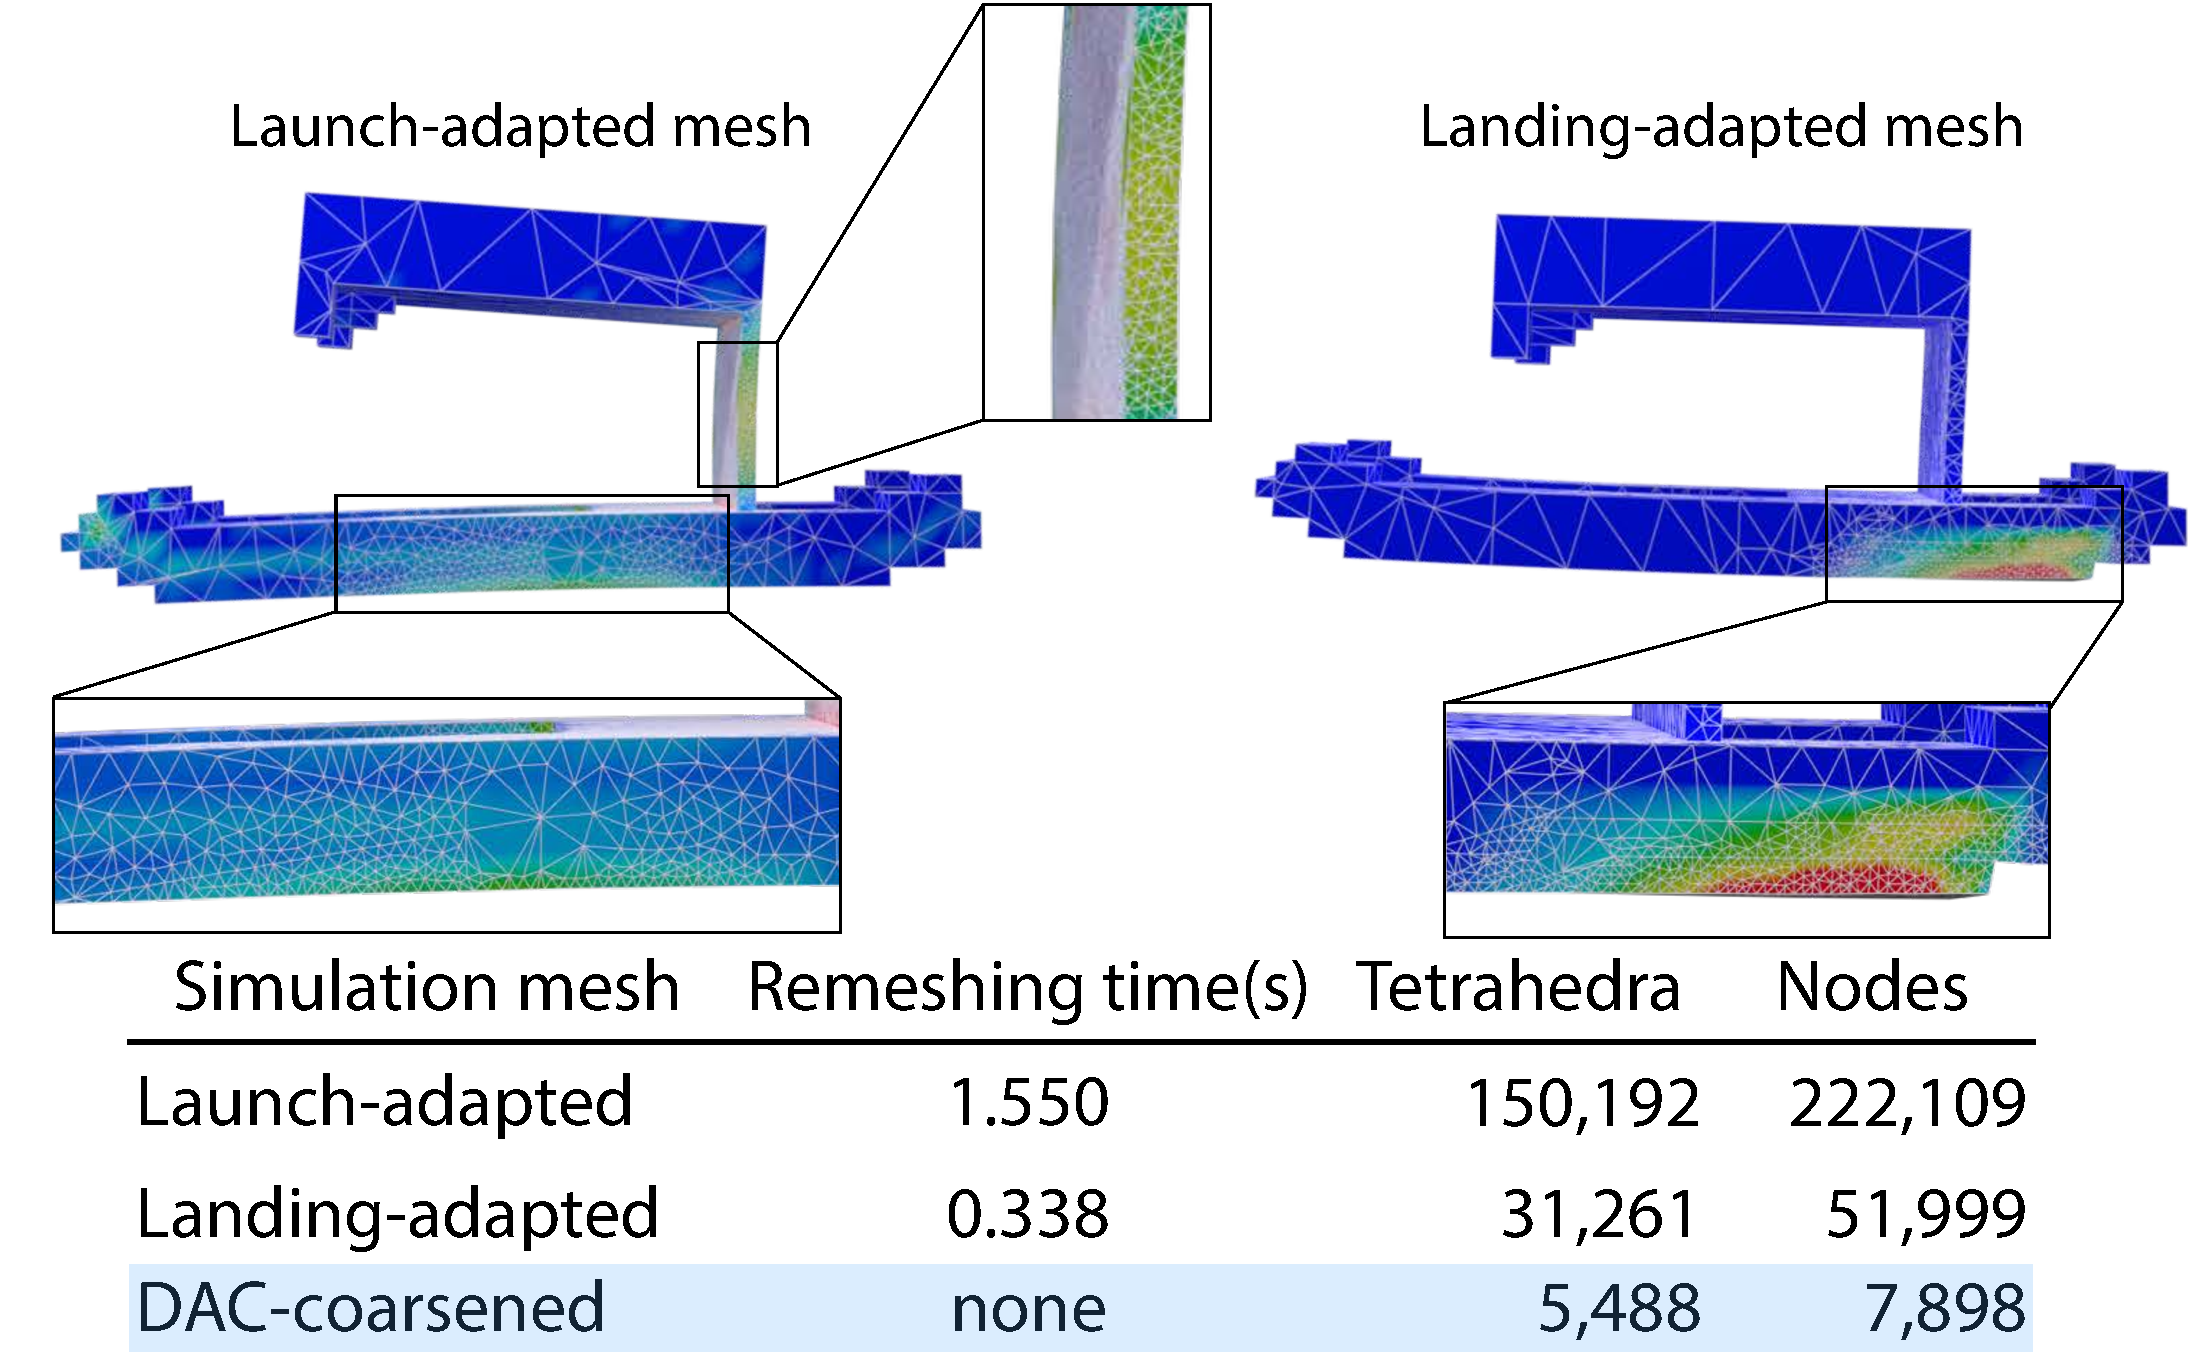
\includegraphics[width=0.7\columnwidth]{./figs/Adaptive_Meshing}	
	\caption{Comparing adaptivity and coarsening. A tetrahedral model of a jumper is adaptively remeshed to capture input stress fields from its launch and landing states. We compare the resulting element and node counts to our DAC-coarsened model. We set the minimum edge length for remeshing to one that was experimentally found to yield convergent numerical results.}
	\label{fig:adaptiveMeshing}
\end{figure}

\emph{Adaptive meshing} allows us to reduce element counts in material regions where refinement is less critical.
Let us ignore the difficulty of implementing adaptive meshing and the per time step cost to remesh. Even so, adaptive meshes are challenging in our setting. We model objects that undergo rapidly changing boundary conditions and globally varying stress fields due to contacts, loading and impacts. Adaptive meshing in our setting must then, necessarily, feature high numbers of elements to capture these details. See Figure~\ref{fig:adaptiveMeshing}. Here, using our experimentally validated, accurate element edge length as adaptive meshing threshold, our tetrahedral mesh contains 6.5X to 28X more nodal DoFs than our corresponding DAC-coarsened mesh. The DAC-coarsened mesh is likewise simpler to implement and has no per time step computational cost. 

\emph{Reduced models} utilizing linear modes~\cite{James:2002:DDR,Hauser:2003:IDU} are widely applied to accelerate dynamic simulations. The key issue here is that linear modal models provide only a \emph{linear} approximation of the deformation space leading to inaccurate linearization artifacts, 
such as swelling during rotation;
see Figure~\ref{fig:modalModels}. Optimized quadrature approaches, in turn, can afford efficient integration of non-linear forcing functions, but do not alleviate these artifacts~\cite{An:2008:OCE} when relying on an underlying modal deformation space.
Finally, nonlinear modal models~\cite{Barbic:subspace:2005} can alleviate some of these issues but so-far remain challenging to incorporate in the design process in comparison to their linear counterparts~\cite{Chinesta2013}. 

\begin{figure}
	\centering
	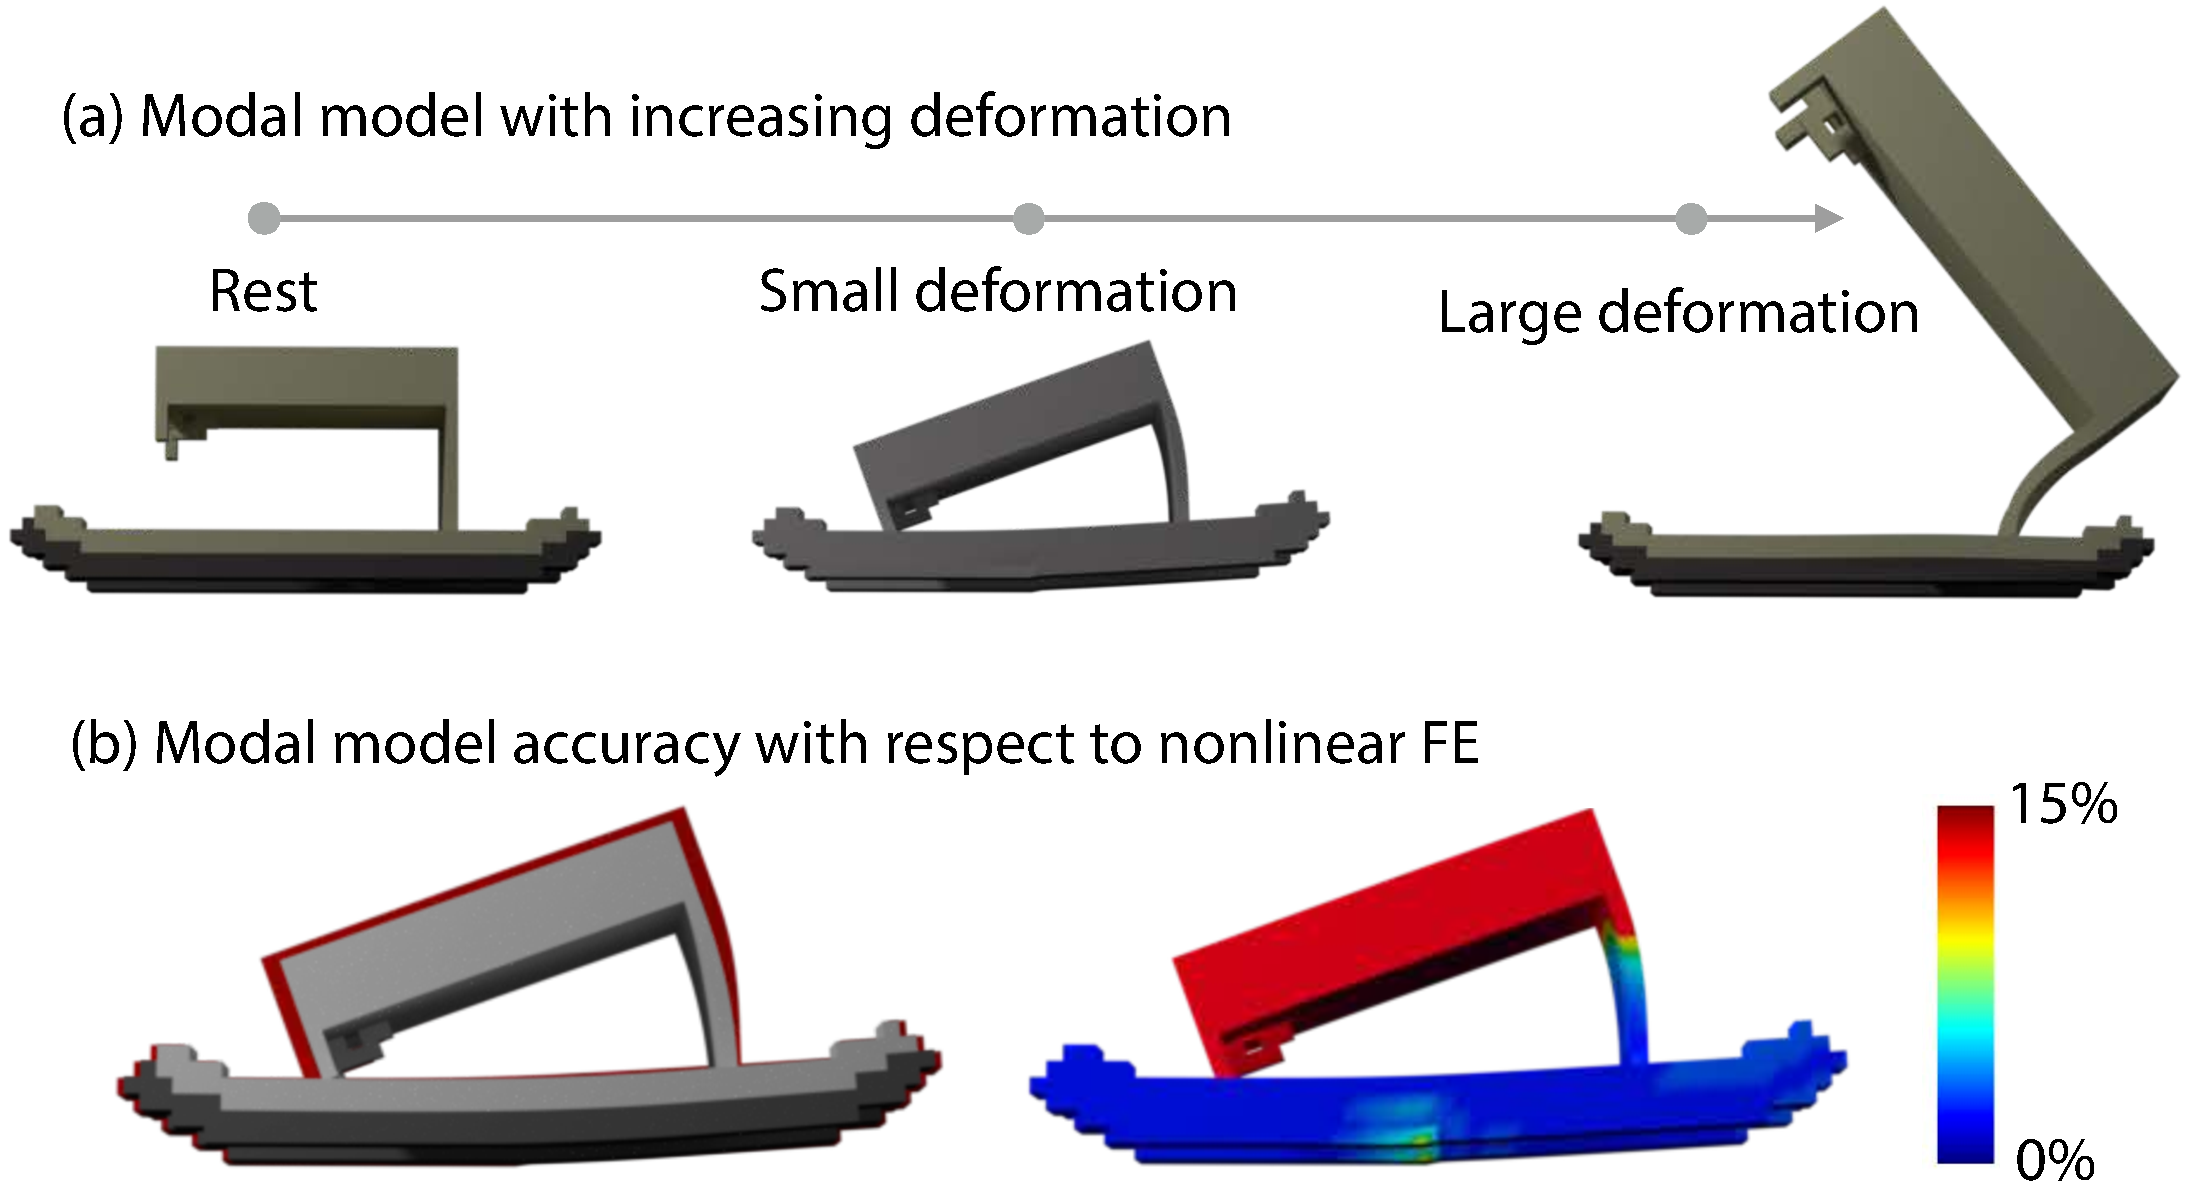
\includegraphics[width=0.7\columnwidth]{figs/Modal_Expansion}
	\caption{Linear modal models suffer from distortion as deformations grow. In (a) we illustrate increasing deformations, left to right, with corresponding inflation errors. Even for smaller deformations, (a) middle, the linear modal model still introduces significant distortions leading to modeling inaccuracies. In (b), left, we overlay simulations of small deformation  performed respectively with the linear modal model (red) and the coarsened nonlinear FE model (grey); and, on the right, evaluate accuracy of the modal model. During simulation, even these smaller deformations introduce inaccuracies in the modal model due to element inflation; here up to 13.7\%.} 
	\label{fig:modalModels}	
\end{figure}

We begin by observing that \emph{numerical coarsening} offers an exciting alternative for efficient yet predictive FE modeling. Coarsening methods effectively apply coarse resolution FE meshes as reduced DoF models and then seek material models that reproduce the behavior of a high-resolution FE counterpart. Analytical solutions for coarsening have been developed for linear material models (models where the stress varies linearly with strain)~\cite{Kharevych:2009cg,Nesme:2009:PTE,Torres:2016:HIC}.
Due to this linear assumption, and similarly to the linear modal models discussed above, we find them difficult to apply for the accurate modeling of the nonlinear materials required for 3D-printed objects.
Even more recently, data-driven coarsening strategies~\cite{chen2015:ddfem} have been proposed to overcome the linear limitation of prior work. Unfortunately, while coarsening offers promise, prior work, to our knowledge, does not account dynamic effects, inertial properties, nor material damping characteristics.
As we see in Figure~\ref{fig:coarse}, this causes even the most recent, nonlinear, data-driven coarsening approaches to produce highly inaccurate dynamic simulations.

Building on the promise of coarsening techniques and inspired by recent developments in frequency matching for plausible computer animation~\cite{Li:2014:SEE,BinWang:2015fx}, we develop a new, dynamics-aware coarsening (DAC) method that, in contrast to prior approaches, provides well-over an order-of-magnitude performance enhancement, while maintaining fabrication-level accuracy when modeling highly dynamic motions subject to frictional contact. Our method does so without complex substructuring, does not require adaptive remeshing, accounts for dynamic effects including damping, and does not introduce prohibitive linear modeling artifacts and so is applicable to a wide selection of nonlinear constitutive models for 3D-printed materials.  

\subsection{Impact Response for Elastic Materials}
Even with a suitably accurate FE solution to model \emph{material} dynamics, accurate impact response for elastic materials on collision remains highly challenging.  To capture the bounces and rebounds of elastic mechanisms coming into contact with the ground - consider for example the heel strike of a sneaker - we need to get this right. State-of-the-art, implicit time-stepping methods for FEM with contact solve variational forms of time-steppers, e.g., variational Implicit Newmark, subject to additional, fully implicit contact and friction forces~\cite{Kane:1999kr,Pandolfi:2002ik}. 
These form so-called nonsmooth or \emph{complementarity} integrators. 


\begin{figure}
	\centering
	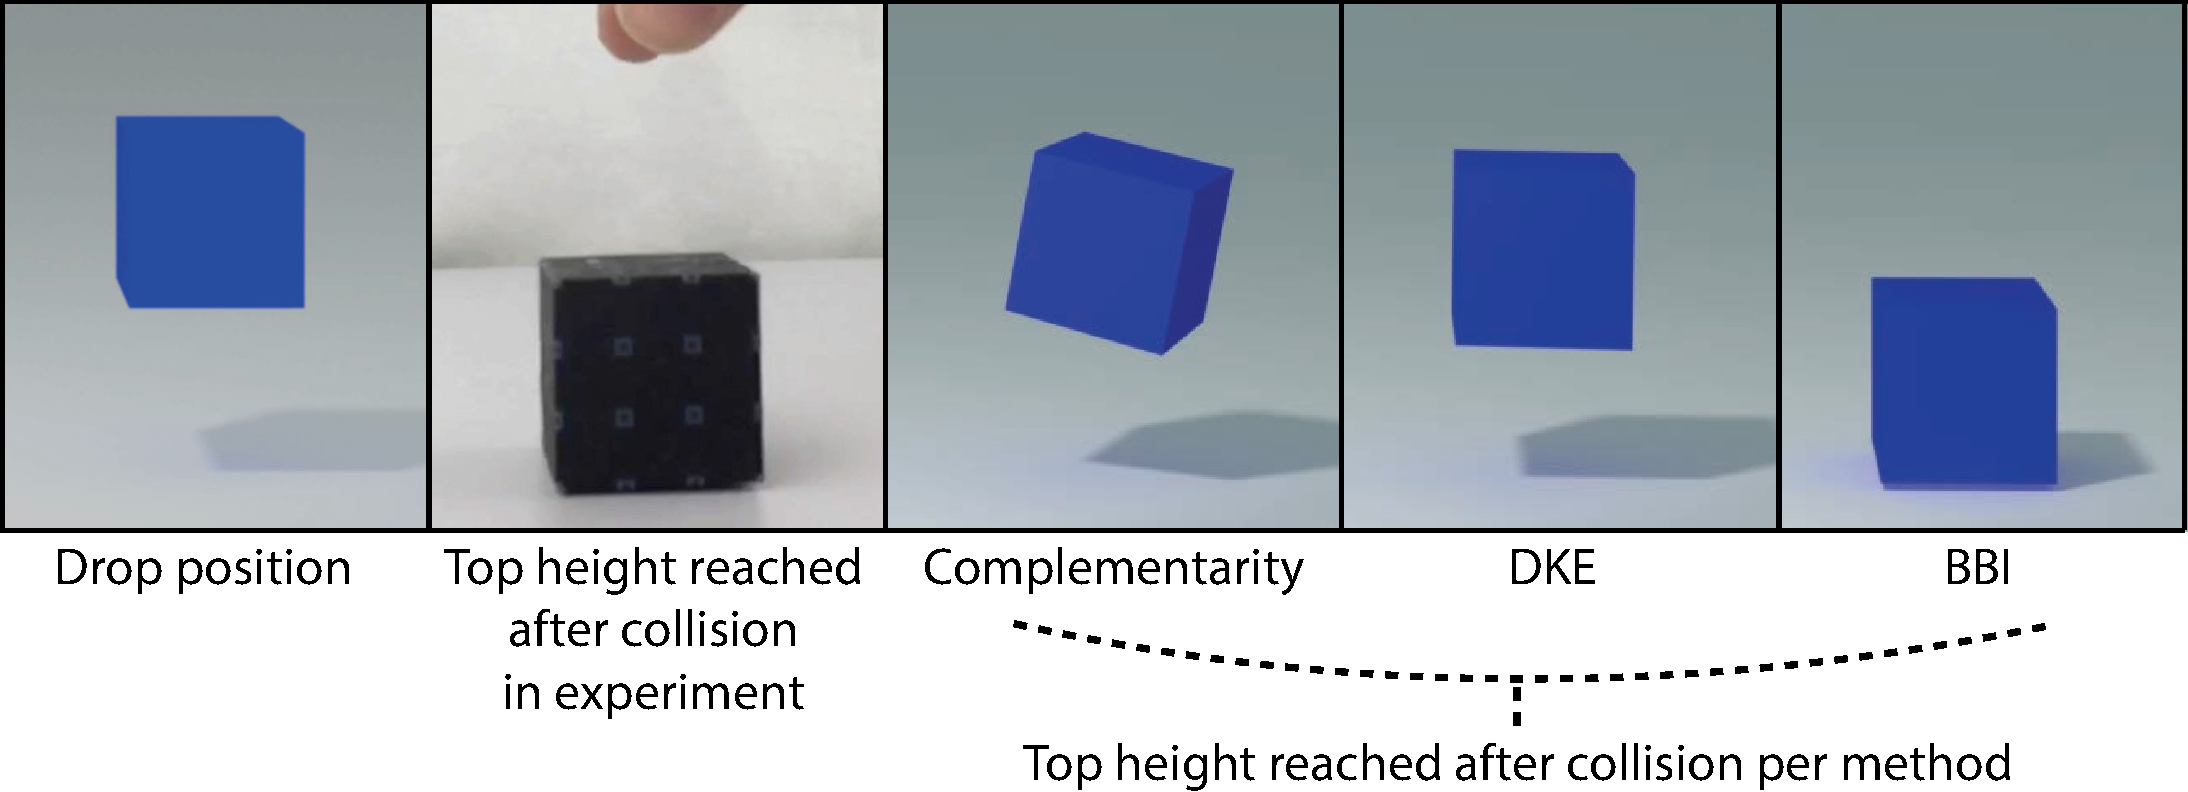
\includegraphics[width=0.8\columnwidth]{figs/Figure_2_BBI}	
	\caption{Comparison of complementarity Newmark integration, DKE Stabilization and our BBI model for the impact resolution of an elastic, 3D-printed block. BBI closely matches the maximum rebound height achieved by the experimental result while both the Complementarity and DKE methods overestimate the rebound significantly.}
	\label{fig:BBI_block_compare}
\end{figure}

However, these complementarity integrators have two well-known flaws~\cite{Deuflhard:2008fu}: (1) these methods can yield spurious oscillations on the contact boundaries and (2) the effective impact response of these methods is too energetic. Effectively the normal velocity on impact along the elastic boundary should be dissipated completely. Instead, complementarity methods with Newmark will generate an entirely incorrect elastic restitution; see Figure~\ref{fig:BBI_block_compare}. To address these problems~\citet{Deuflhard:2008fu} introduced the now-standard DKE contact-stabilization step to filter contact response with projection. In the limit, DKE makes the impact-response model consistent,
while in FE codes it is applied as an effective strategy to recover from the well-known limitations of implicit integration with impact. However, it remains widely acknowledged that the right-way to accurately model high-speed collision response with implicit FE remains an open question at this time - not only in graphics - but more broadly in scientific computing as well. As an example consider Figure~\ref{fig:BBI_block_compare} where we see that both the complementarity model \emph{and} the DKE filter produce different but equally incorrect predictions of the response of a stiff elastic block dropped on the floor. Here we offer a new, Boundary-Balancing Impact (BBI) model for FE that gains us accurate prediction of impact response for the stiff 3D-printed materials we focus on here; see Figure~\ref{fig:BBI_block_compare}.

\subsection{Summary and Contributions}
High-fidelity simulation methods for elastodynamics are too slow for use in fabrication design tasks while existing strategies to reduce the simulation cost of elastica (including adaptive, reduced and coarsened models) are too inaccurate and/or too expensive to employ. Finally, existing FE models for simulating elastic collision and rebound miss critical compliance coupling in the filter stage.

We have exposed and analyzed the limitations of simulation methods for the predictive modeling of elastodynamics at rates sufficient for fabrication design optimization. Next, we develop our \emph{Dynamics-Aware Coarsening} (DAC) method to address this need {(\S3)}. DAC jointly identifies \emph{and} predictively simulates fabricated materials. To address current limitations in FE collision-response filtering we then introduce our \emph{Boundary Balancing Impact} (BBI) model {(\S4)}. 
We then validate these contributions by comparing simulated results generated by DAC and BBI with real-world results experimentally obtained from a range of compliant 3D-printed jumping and throwing mechanisms that flip, throw projectiles, jump onto obstacles and jump over walls (\S5).
\section{Simulation Preliminaries}
\begin{figure}
	\centering
	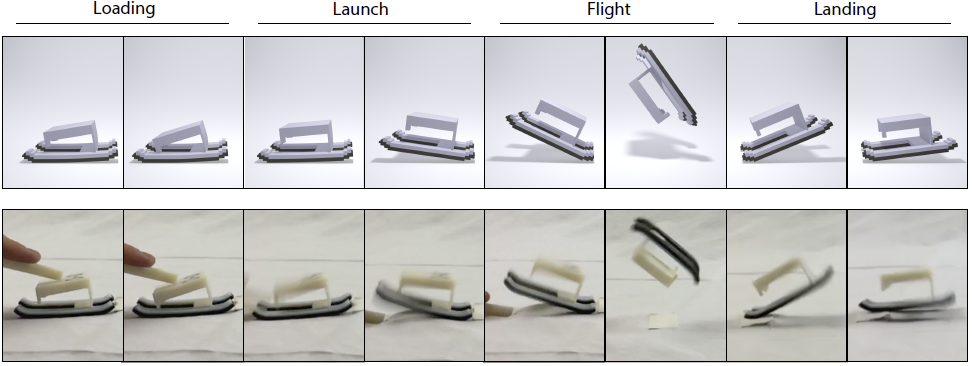
\includegraphics[width=0.99\textwidth]{images/dynPhase.png}
	\caption{Bottom: the dynamic behavior of a 3D-printed, elastic jumping mechanism in experiment. Top: our DAC-coarsening combined with our BBI impact model generate a simulation that predictively captures this experimental behavior at rates 79X faster than state-of-the-art FEM.}
	\label{fig:simulationStage}
\end{figure}
\label{sec:simPrelim}
Accurate time-varying tracking of energy dissipation is key to accurate dynamic simulation~\cite{Marsden:2001dj} and so we rely on implicit Newmark time integration, a discrete variational integrator~\cite{Kane:2000dw} with consistent high-quality energy tracking. 
We experimented with other integrators, including linearly implicit Newmark, Implicit Euler, and BDF2, but found them to be wanting in either stability or energetic behavior; see our Supplemental for details.
\subsection{Discrete Model} We begin with a standard elastic material model for 3D printed materials.
To capture stiff elastic response of 3D-printed materials we use the neo-Hookean material model, augmented with Rayleigh damping to capture transient dissipation of vibrations, and discretize with second order, hexahedral finite elements. We start with a second-order, implicit Newmark %($\gamma=1/2,\beta=1/4$) 
time discretization 

\begin{align}
\vc M \vc \delta^{t+1} &= \vc b^t +  \tfrac{h^2}{4} \vc F(\vc q^{t+1}) -\tfrac{h^2}{4} \vc D(\vc q^{t+1}) \vc v^{t+1},
\label{eq:newmark_free}
%
\end{align}
\begin{align}
\begin{split}
\vc q^{t+1} &= \vc q^t + \vc \delta^{t+1},\\
\vc v^{t+1} &= \tfrac{2}{h} \vc \delta^{t+1} - \vc v^t,
\end{split}
\label{eq:newmark_free_update}
\end{align}
where
\begin{align}
\vc b^t = h \vc M \vc v^t + \tfrac{h^2}{4} \vc F( \vc q^t) -\tfrac{h^2}{4} \vc D( \vc q^t) \vc v^t,
\label{eq:newmark_predictor}
\end{align}
$h$ is the timestep size, $\vc F(\cdot)$ is the internal force vector, $\vc D(\cdot) = a \vc M + b \vc K(\cdot)$, 
with $a,b \in \mathbb{R}^+$ is the Rayleigh damping matrix, $\vc M$ is the stiffness-consistent mass-matrix~\citep{Belytschko:2013tz},
$\vc K(\cdot) = -\nabla \vc F(\cdot)$ is the tangent stiffness matrix, 
and $\vc q, \vc v \in \mathbb{R}^{3n}$ are respectively the nodal position and velocity vectors. In the absence of dissipative forces this method is symplectic and momentum preserving~\citep{Kane:2000dw}.
With dissipation we find that integration gives us accurate bookkeeping of system energy at comparable cost to implicit Euler. 

\subsection{Material Parameters}
No matter how good our energy bookkeeping, the overall fidelity of our method is critically determined by the accuracy of the material parameters we select. While many material parameters are reported in the literature, there remains large and significant variation in these values across 3D-print batches, printing orientations and curings; see \S5.
For predictive simulation we need to identify these values. In addition, we must model dissipation requiring us to determine unreported damping properties; e.g., $a$ and $b$ in the Rayleigh model. Finally, as discussed below and complicating matters even further, these material parameters are discretization dependent at non-convergent spatial resolutions. In the next section we will detail our DAC model to capture dynamic deformation, stiffness and damping at coarsened spatial resolutions.

\subsection{Contact and Friction} For contact we need to model nonpenetration constraints and frictional contact forces that resist sliding along interfaces. 
Contacts are between object parts or between a part and a fixed boundary such as the ground.  At each time step we apply continuous collision detection to the predicted trajectory to gather contact constraints into a contact set $\mathcal C$. 

To simplify the following, for each such contact $k \in \mathcal C$, the relative acceleration between material points $\vr x_i$ and $\vr x_j$ (at contact $k$) can be expressed via the map $\vc \Gamma_k: \dot{\vc q} \rightarrow \dot{\vr x}_i - \dot{\vr x}_j$. See our Supplement
for details on construction of $\vc \Gamma_k$. If $\vr y \in \mathbb{R}^3$ is a force applied to point $\vr x_i$, and an equal but opposite force is applied to point $\vr x_j$, then $ \vc \Gamma_k ^T \vr y$ is the resulting generalized force applied to the contacting system.

In turn, points in contact apply an equal and opposite force along their shared, unit-length normal $\vr n_k \in \mathbb{R}^3$.  In global coordinates this is equivalent to applying a force of magnitude $\bar{\alpha}_k \in \mathbb{R}^+$ along a generalized normal 
\begin{equation}
\vc n_k = \vc \Gamma_k^T \vr n_k \in \mathbb{R}^{3n},
\end{equation}
to the system. The subspace of generalized normal directions
\begin{equation}
\label{eq:N}
\vc N = (\vc n_1 ... \vc n_{|\mathcal C|})
\end{equation}
then forms a basis for contact forces. Concatenating the corresponding force magnitudes in  
$\alpha = (\bar{\alpha}_1, ..., \bar{\alpha}_{|\mathcal{C}|})^T$, the total contact force applied in the system is then $\vc N \alpha$. 

Friction forces lie in the tangent plane orthogonal to the contact normal. At each contact $k$ we sample an orthogonal pair of unit length vectors from the tangent plane. The $3\times2$ matrix composed column-wise of these samples is given by $\vr T_k$ so that a friction force, $\vr f_k \in \mathbb{R}^3$, applied at a contact $k$, lies in the span of $\vr T_k$ with $\vr f_k = \vr T_k \bar{\beta}_k$, where each $\bar{\beta}_k \in \mathbb{R}^2$ gives the frictional response coefficients at contact $k$.

The total friction force applied to the system at each contact $k$ must be equal and opposite and is $\vc f_k = \vc \Gamma_k^T \vr T_k \bar{\beta}_k$. 
The generalized basis for a friction force at contact $k$ is then 
\begin{equation}
\vc T_k = \vc \Gamma_k^T \vr T_k \in \mathbb{R}^{3n \times 2}.
\end{equation}
We build the corresponding subspace of generalized tangent directions,
\begin{equation}
\vc T = ( \vc T_1 ... \vc T_{|\mathcal C|})
\end{equation}
and form the corresponding vector of frictional force coefficients as $\beta = ( \bar{\beta}^T_1,  ... , \bar{\beta}^T_{|\mathcal C|})^T$.
The total friction force on the system is then $\vc T \beta$.

Contact and friction forces can be inexpensively modeled explicitly~\citep{Belytschko:2013tz} but this introduces instabilities and nonphysical oscillations on boundaries even at small time step for stiffer materials~\cite{Deuflhard:2008fu}. Thus FEM state-of-the-art generally turns to implicit time-integration for efficient contact force modeling. 

\citet{Kane:1999kr} proposed the now standard nonsmooth-Newmark method for contact modeling. 
This is a fully implicit time-stepping model that couples frictional contact with internal energies and forcing in each solve.
\begin{align}
\begin{split}
\vc M \vc \delta^{t+1} &= \vc b^t +  \tfrac{h^2}{4} \vc F(\vc q^{t+1}) -\tfrac{h^2}{4} \vc D(\vc q^{t+1}) \vc v^{t+1} + \tfrac{h^2}{2} \vc N \alpha +  \tfrac{h^2}{2}  \vc T \beta.
\label{eq:newmark_contact_implicit}
\end{split}
\end{align}
Note that here, unlike internal forces, contact forces are evaluated solely at the time step endpoint to ensure dissipation.
Next, to fully define the time stepper, consistency conditions are required for contact and friction forces. 

Enforcing the complementarity model for contact requires contact forces to balance along boundaries 
\begin{align}
\begin{split}
0 \leq \alpha \perp \vc N^T \delta^{t+1} \geq 0,
\label{eq:contact_conditions}
\end{split}
\end{align}

Friction in turn is modeled with the {\em Maximal Dissipation Principle}, requiring friction to maximize the rate of negative work done at each contact, $- \vr f_k^T \dot{\vr x}$. The total dissipation performed by friction is then 
\begin{align}
\sum_{k \in \mathcal{C}} \bigl(- \vr f_k^T \dot{\vr x}_k \bigr) =  -\Bigl[\sum_{k \in \mathcal{C}} \vr f_k^T  \vc \Gamma_k \Bigr] \dot{\vc q} =  - \beta^T \vc T^T \dot{\vc q}.
\end{align}
Then, maximizing the Coulomb-constrained dissipation simultaneously at \emph{all} contact points, with the implicit Newmark discretization~\cite{Pandolfi:2002ik}, gives us the final condition for our numerical integration
\begin{align}
\begin{split}
\min_{\beta} \{ \beta^T \vc T^T (\tfrac{2}{h} \delta^{t+1} - \vc v^t) : \mu_k \bar{\alpha}_k \geq \|\bar{\beta}_k\|, \> \forall k \in \mathcal{C} \},
\label{eq:max_diss_transform}
\end{split}
\end{align}
where $\mu_k$ is the local friction coefficient at contact $k$.

Taken together stepping this implicit \emph{complementarity} Newmark integrator with (\ref{eq:newmark_predictor}), (\ref{eq:newmark_contact_implicit}), (\ref{eq:contact_conditions}), (\ref{eq:max_diss_transform}) and (\ref{eq:newmark_free_update}) provides predictive simulation at slower speeds of contact. For higher speed contacts and impacts, the remaining challenge lies in stabilizing contact stresses, velocities and displacements~\cite{Deuflhard:2008fu} to ensure that simulated objects' bounces and rebounds consistently match with their real-world counterparts. 
In Section \ref{sec:BBI} we will address this issue with a new impact model for FE simulation. First, however, we address our fundamental scaling problem: how can we gain 
accurate dynamic simulation without being bottlenecked by systems too large to solve quickly per time step?
\section{Dynamics-Aware Coarsening}
\label{sec:DAC}
We couple numerical coarsening with parameter acquisition.
Our DAC method computes \emph{numerical} stiffness parameters for the nonlinearly elastic, Neohookean material model, and damping parameters for the Rayleigh damping model so that, when applied to the coarsened simulation mesh, the dynamic behavior of a high-resolution simulation is preserved.

\begin{figure}
	\centering
	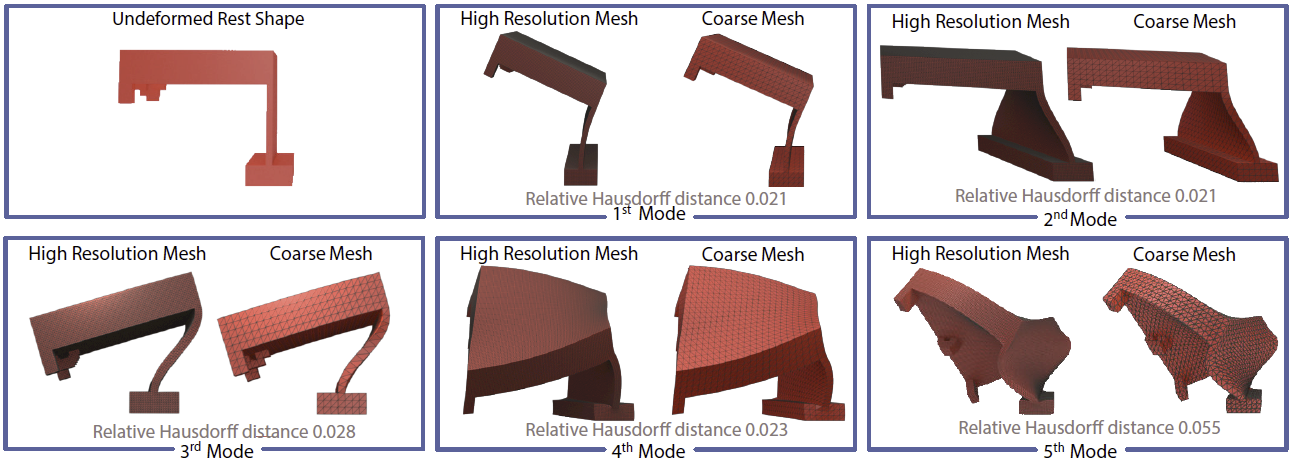
\includegraphics[width=0.95\columnwidth]{images/modeFit.png}
	\caption{Dynamics-aware coarsening (DAC) coarsens meshes to capture deformation with calibrated stiffness. We observe FE meshes capture accurate deformation modes up to a quite coarse resolution. However, these same coarse meshes suffer from numerical stiffening (see Figure~\ref{fig:numerical_stiffness}). We design coarse mesh FE models by matching both significant deformation modes (above) and their captured material response (see Figures~\ref{fig:error} and \ref{fig:vibration_match}) to obtain efficient and predictive coarse-mesh FEM simulations of dynamics. }
	\label{fig:defo_and_frequency_match}
\end{figure}

Because the goal of DAC is to replicate the dynamic behavior of a high-resolution simulation, we focus on creating a coarse mesh which captures both the large-scale deformation modes, and the corresponding natural frequencies of the high-resolution mesh. We do this in two stages. First, we produce a coarse hexahedral mesh that can replicate the large scale deformation modes of our high-resolution mesh. Second, we compute material and damping parameters that yield matching fundamental frequencies for each mode shape on this coarse mesh.

\begin{figure}
	\centering
	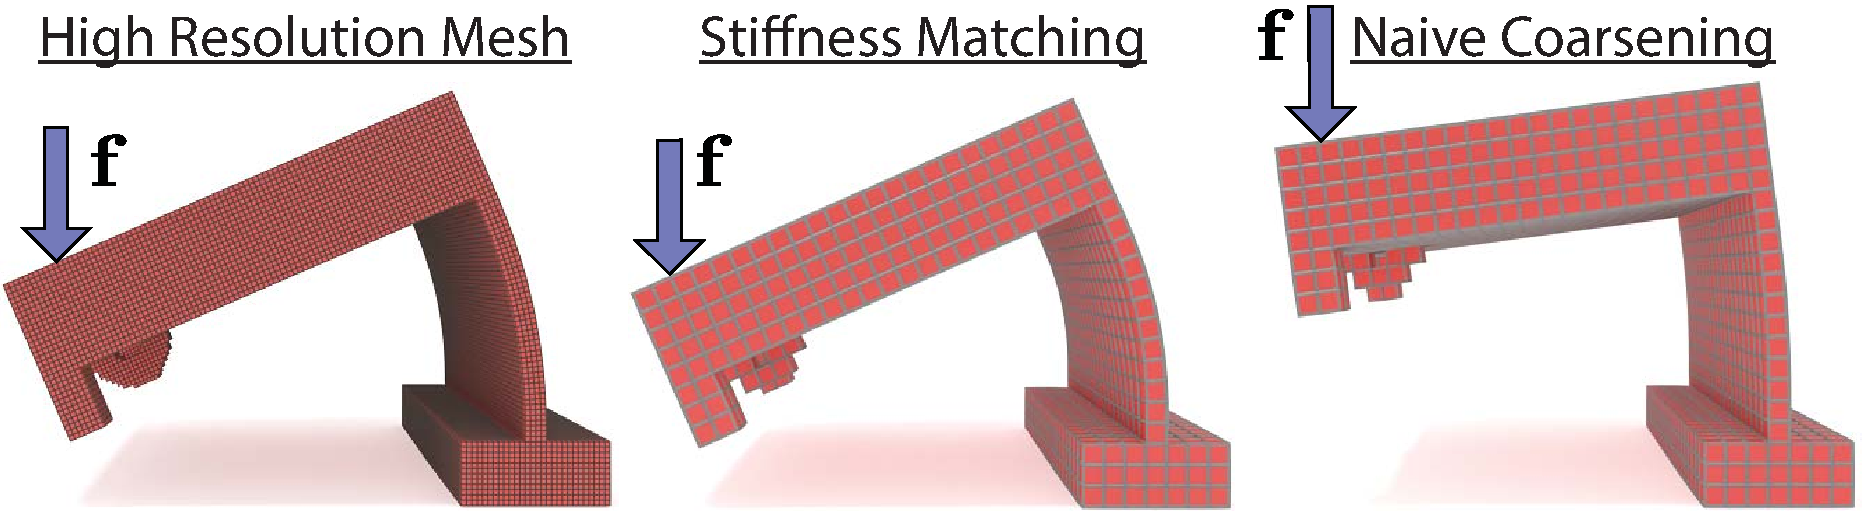
\includegraphics[width=0.7\textwidth]{figs/stiffness.pdf}
	\caption{Static Deformation Test. We apply an identical load to three meshes with the same model geometry. With the same material parameters, a high-resolution mesh (left) is effectively 2.5x softer than the corresponding coarse mesh (right). Applying our captured numerical Young's modulus to the coarse mesh (middle) regains the correct deformation of the original, high-resolution mesh on the left.}
	\label{fig:numerical_stiffness}
\end{figure}

\subsection{Geometric Coarsening}
DAC uses an iterative procedure {to create the} coarse mesh while maintaining mode shapes. We initialize our mesh to a coarse hexahedral discretization of the starting geometry, $\vc q^0$, and then subdivide recursively until we reach a convergent mesh resolution. We then solve the generalized mass-PCA system 
\begin{align}
\vc K(\vc q^0) \vc q = \lambda \vc M \vc q
\end{align}
for the dominant shape modes of the convergent system and then coarsen via bisection 
with mass-PCA until we reach a maximally coarse mesh that matches the dominant four shape modes to tolerance. We use a relative geometric difference of $5\%$ (Hausdorff distance) as our tolerance threshold. Typically this is a short validation step as even the coarsest meshes generally satisfy this criteria (Figure~\ref{fig:defo_and_frequency_match}).

\subsection{Material Parameter Fitting}  
Our geometric coarsening ensures that our DAC mesh captures significant deformation modes of our design accurately. However, when simulated, these same coarse meshes suffer from \emph{numerical stiffening} -- an increase in effective stiffness and damping as a consequence of decreased mesh resolution; see Figure~\ref{fig:numerical_stiffness}. This leads to unacceptably inaccurate simulated trajectories no matter how we simulate this system. Regaining predictive stiffness and damping by refining the discretization would take us back to intractable mesh sizes; see Figure~\ref{fig:adaptiveMeshing}.
Rather than refine, we keep our coarse mesh (as we have already ensured that our geometry is resolved there) and instead calibrate its frequency spectrum to directly match experiment. 

To do this, we rescale our coarse model stiffness so that its fundamental frequency matches an observed frequency. As we will see below, this simple analysis sufficiently recovers effective stiffness and damping to regain a predictive 
nonlinear simulation with our coarse mesh. 

From the geometric coarsening step above, we retain the numerical eigenvalues, $\lambda_i^0$, of our coarse mesh with corresponding deformation modes $m_i$ approximated linearly by the damped harmonic oscillator~\cite{Anonymous:TmbCyHDJ} 
\begin{align}
\ddot m_i = -(a + b \lambda_i ) \dot m_i - \lambda_i m_i,
\end{align}
or equivalently 
\begin{align}
\begin{split}
m_i(t) = &A_i\exp(-d_i t)\sin(2 \pi f_it+ \theta_i),\\
&f_i = \frac{1}{2\pi}\sqrt{\lambda_i - (\frac{a+ b \lambda_i}{2})^2},\\
&d_i=\frac{1}{2}(a + b \lambda_i),
\label{eq:oscillator}
\end{split}
\end{align} where $a$ and $b$ are Rayleigh Damping parameters and $\lambda_i$ is the $i^{th}$ eigenvalue associated with the $i^{th}$ deformation mode.

\begin{figure}
	\centering
	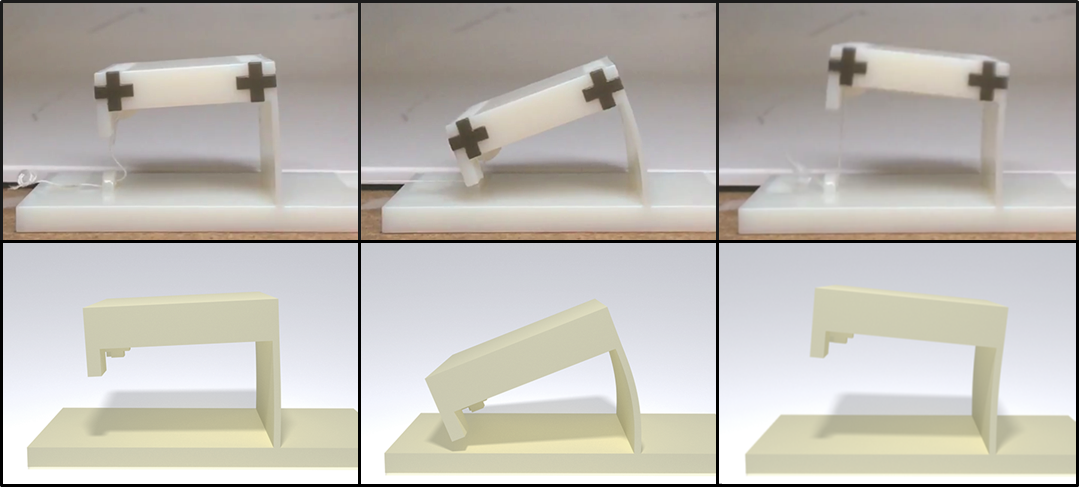
\includegraphics[width=0.6\columnwidth]{images/calibrationfig.png}
	\caption{Top: tracking the oscillations of a 3D-printed calibration rig allows us to measure mesh-dependent stiffness and damping parameters. Bottom: the resulting DAC-simulated frames at corresponding times for visual comparison to the captured motion.}
	\label{fig:calibrationRig}
\end{figure}

We then 3D-print calibration rigs with tracker markings, see e.g., Figure~\ref{fig:calibrationRig}, and capture high-speed video (240 fps) of the rigs vibrating.  
We extract a tracked trajectory $m_t$ of the marker motion from the video capture and solve the inverse harmonics problem~\citep{Mandelshtam:1997gr} to find the printed beam's frequency, $f_t$, and damping, $d_t$, parameters. Setting the tracked $f_t $ and $d_t$ in (\ref{eq:oscillator}) and $a=0$, based on our observation of minimal effective mass-damping, simultaneously retrieves the captured target eigenvalue $\lambda_t$ and the unknown and unreported stiffness damping parameter $b$ required for dynamic simulation. 

With our tracked $\lambda_t$ in hand, our final step is to map the initial material Young's modulus, $E_m$, that we use to compute $\lambda_i^0$ (we set $E_m=1$ throughout)
to a new, \emph{numerical} modulus value, $E_n$.
We seek an $E_n$ that will match the numerical stiffness response of the simulated coarse FE mesh to the captured material response. We do this with a simple argument of fixed proportionality between the principle eigenvalues and the moduli by setting 
\begin{align}
E_n \leftarrow \frac{\lambda_t}{\lambda^0_1}  E_m.
\end{align}
As validation we confirm that our coarsened FE simulations, initialized to the starting calibration pose, with 
Young's modulus set to $E_n$, and stiffness damping set to the measured damping parameter, match both high-resolution simulation and the tracked calibration rig, up to viscosity---which we so far find unnecessary to model; see~\autoref{fig:vibration_match}. 

Note that, in our experiments, increasing the number of mode shapes which must fall below our error threshold of $5\%$  Hausdorff distance does not improve simulation accuracy. Figure~\ref{fig:error} shows a comparison of DAC meshes created using $4$ and $10$ modes for the error threshold. The resulting simulations are indistinguishable from each other and both match measured experimental data equally well. 

In practice we observe that DAC captures object motions containing large contributions from a number of modes. To understand why we see that DAC scaling corrects frequencies of modes well beyond the first, so that, for example, for our plant and walker models, DAC reduces average frequency error across the first 10 modes from 27.1\% to 2.4\%. 

\begin{figure}
	\centering
	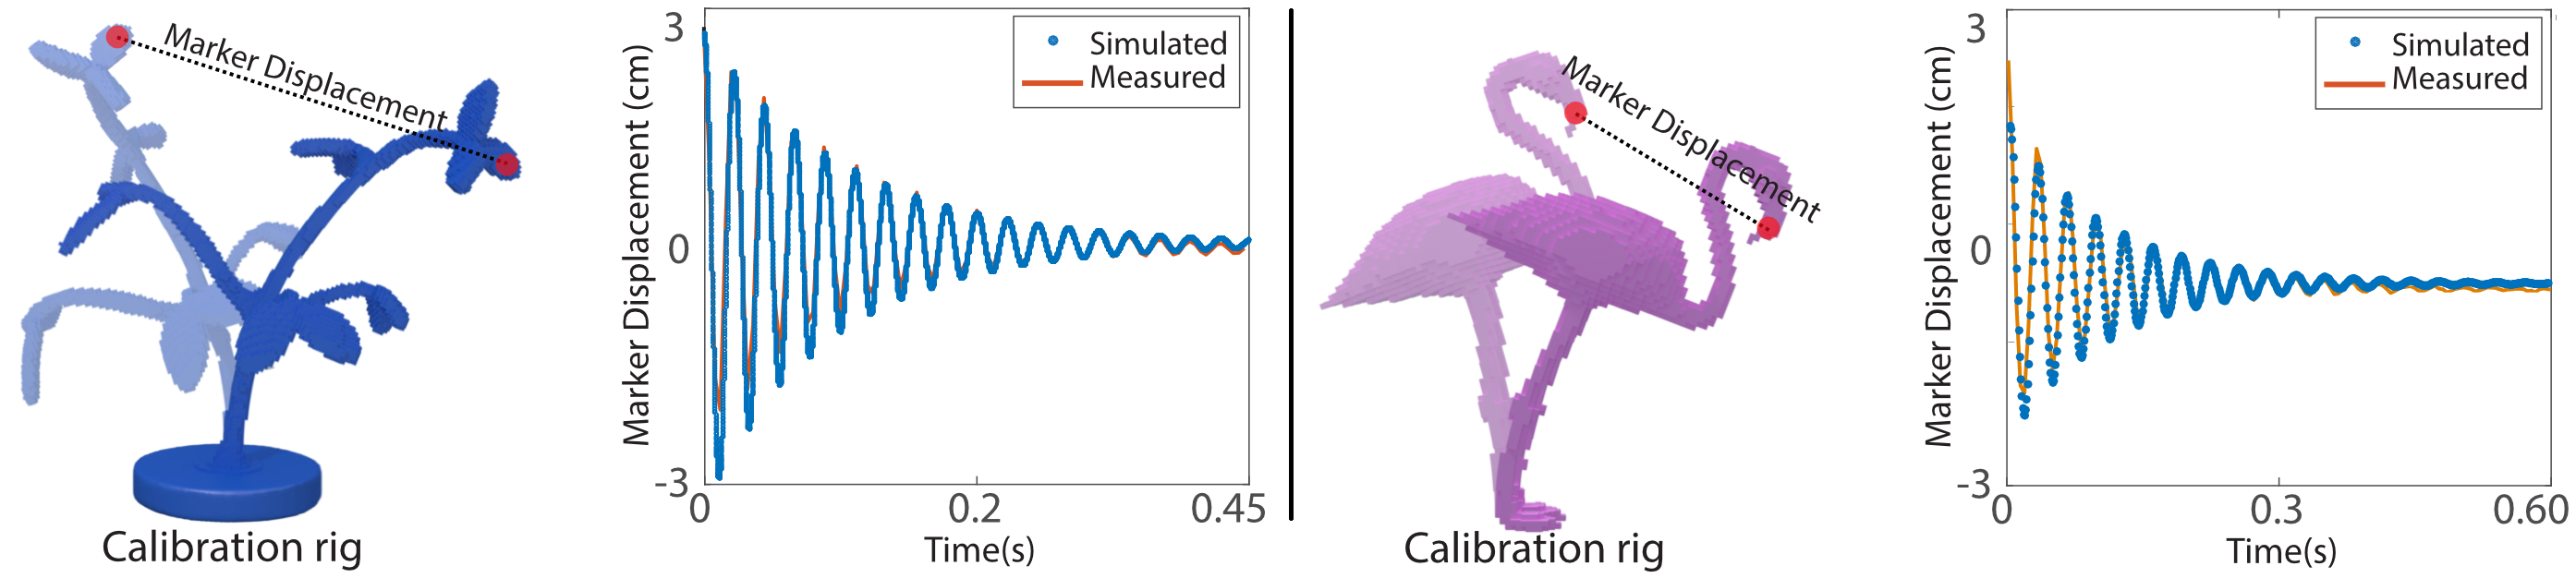
\includegraphics[width=0.9\textwidth]{images/measurePlantEdna.png}
	\caption{Measured and simulated vibrations of the 3D-printed plant (digital material) and 3D-printed flamingo (Rigur RGD450) models (magnify the plots for details of fits).}
	\label{fig:vibration_match_plant}
\end{figure}

\begin{figure}
	\centering
	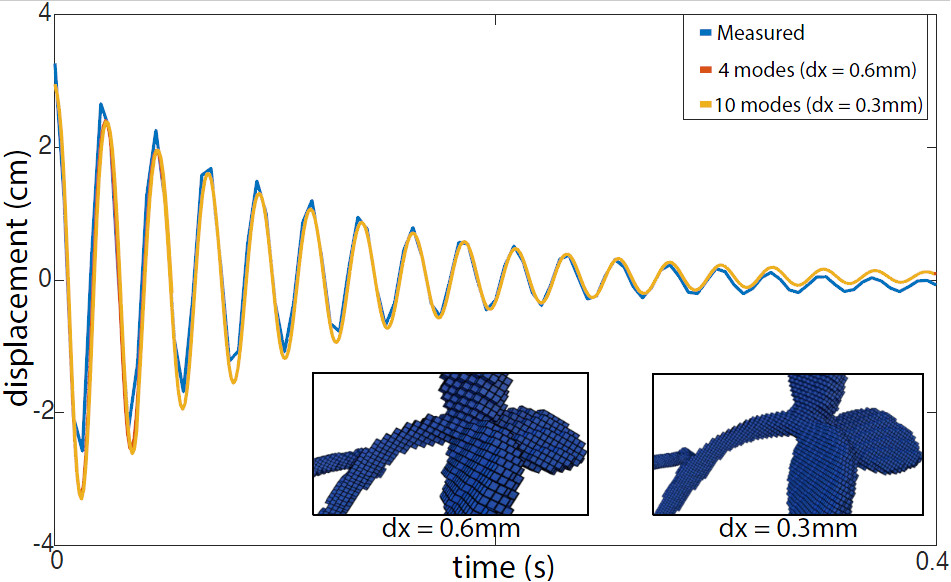
\includegraphics[width=0.6\textwidth]{images/coarseFineVibe.png}
	\caption{DAC coarsening comparison for increasing the number of fitted modes. Our default setting requires less than $5\%$ relative Hausdorff distance up to the $4^{th}$ mode and gives a coarsened FE mesh with $dx=0.6mm$. If we increase the number of modes for our DAC fit to less than $5\%$ relative Hausdorff for up to the $10^{th}$ mode shape, we instead obtain a mesh with $dx=0.3mm$. Note that the resultant simulations for these two DAC meshes are indistinguishable (magnify the plot for detail of fit). }
	\label{fig:error}
\end{figure}

Figure~\ref{fig:vibration_match_plant} shows an example of DAC coarsening applied to plant and flamingo models. With DAC we accelerate the simulation of the time varying deformation of our plant object by 25X while achieving good approximation to the high-resolution simulation mesh; see Figure~\ref{table:suff}. Here Figure~\ref{table:suff} distinguishes between convergent FEM discretizations and accurate FEM discretizations for meshes used in our examples. Convergent discretizations are ones for which the spatial resolution is high enough so that the modal frequencies of the mesh have converged to their final values (changing by less than $1\%$ with respect to previous subdivision). Accurate discretizations are ones for which the resolution of the FE mesh is such that the modal frequencies are within $5\%$ of convergent values. In this paper all results are with respect to the coarser, accurate FE meshes. Even compared to these we achieve speedups of up to 79X. We also note that, if measurement data  is not available, DAC calibration can be carried out using high-resolution simulation data.
\begin{figure}
	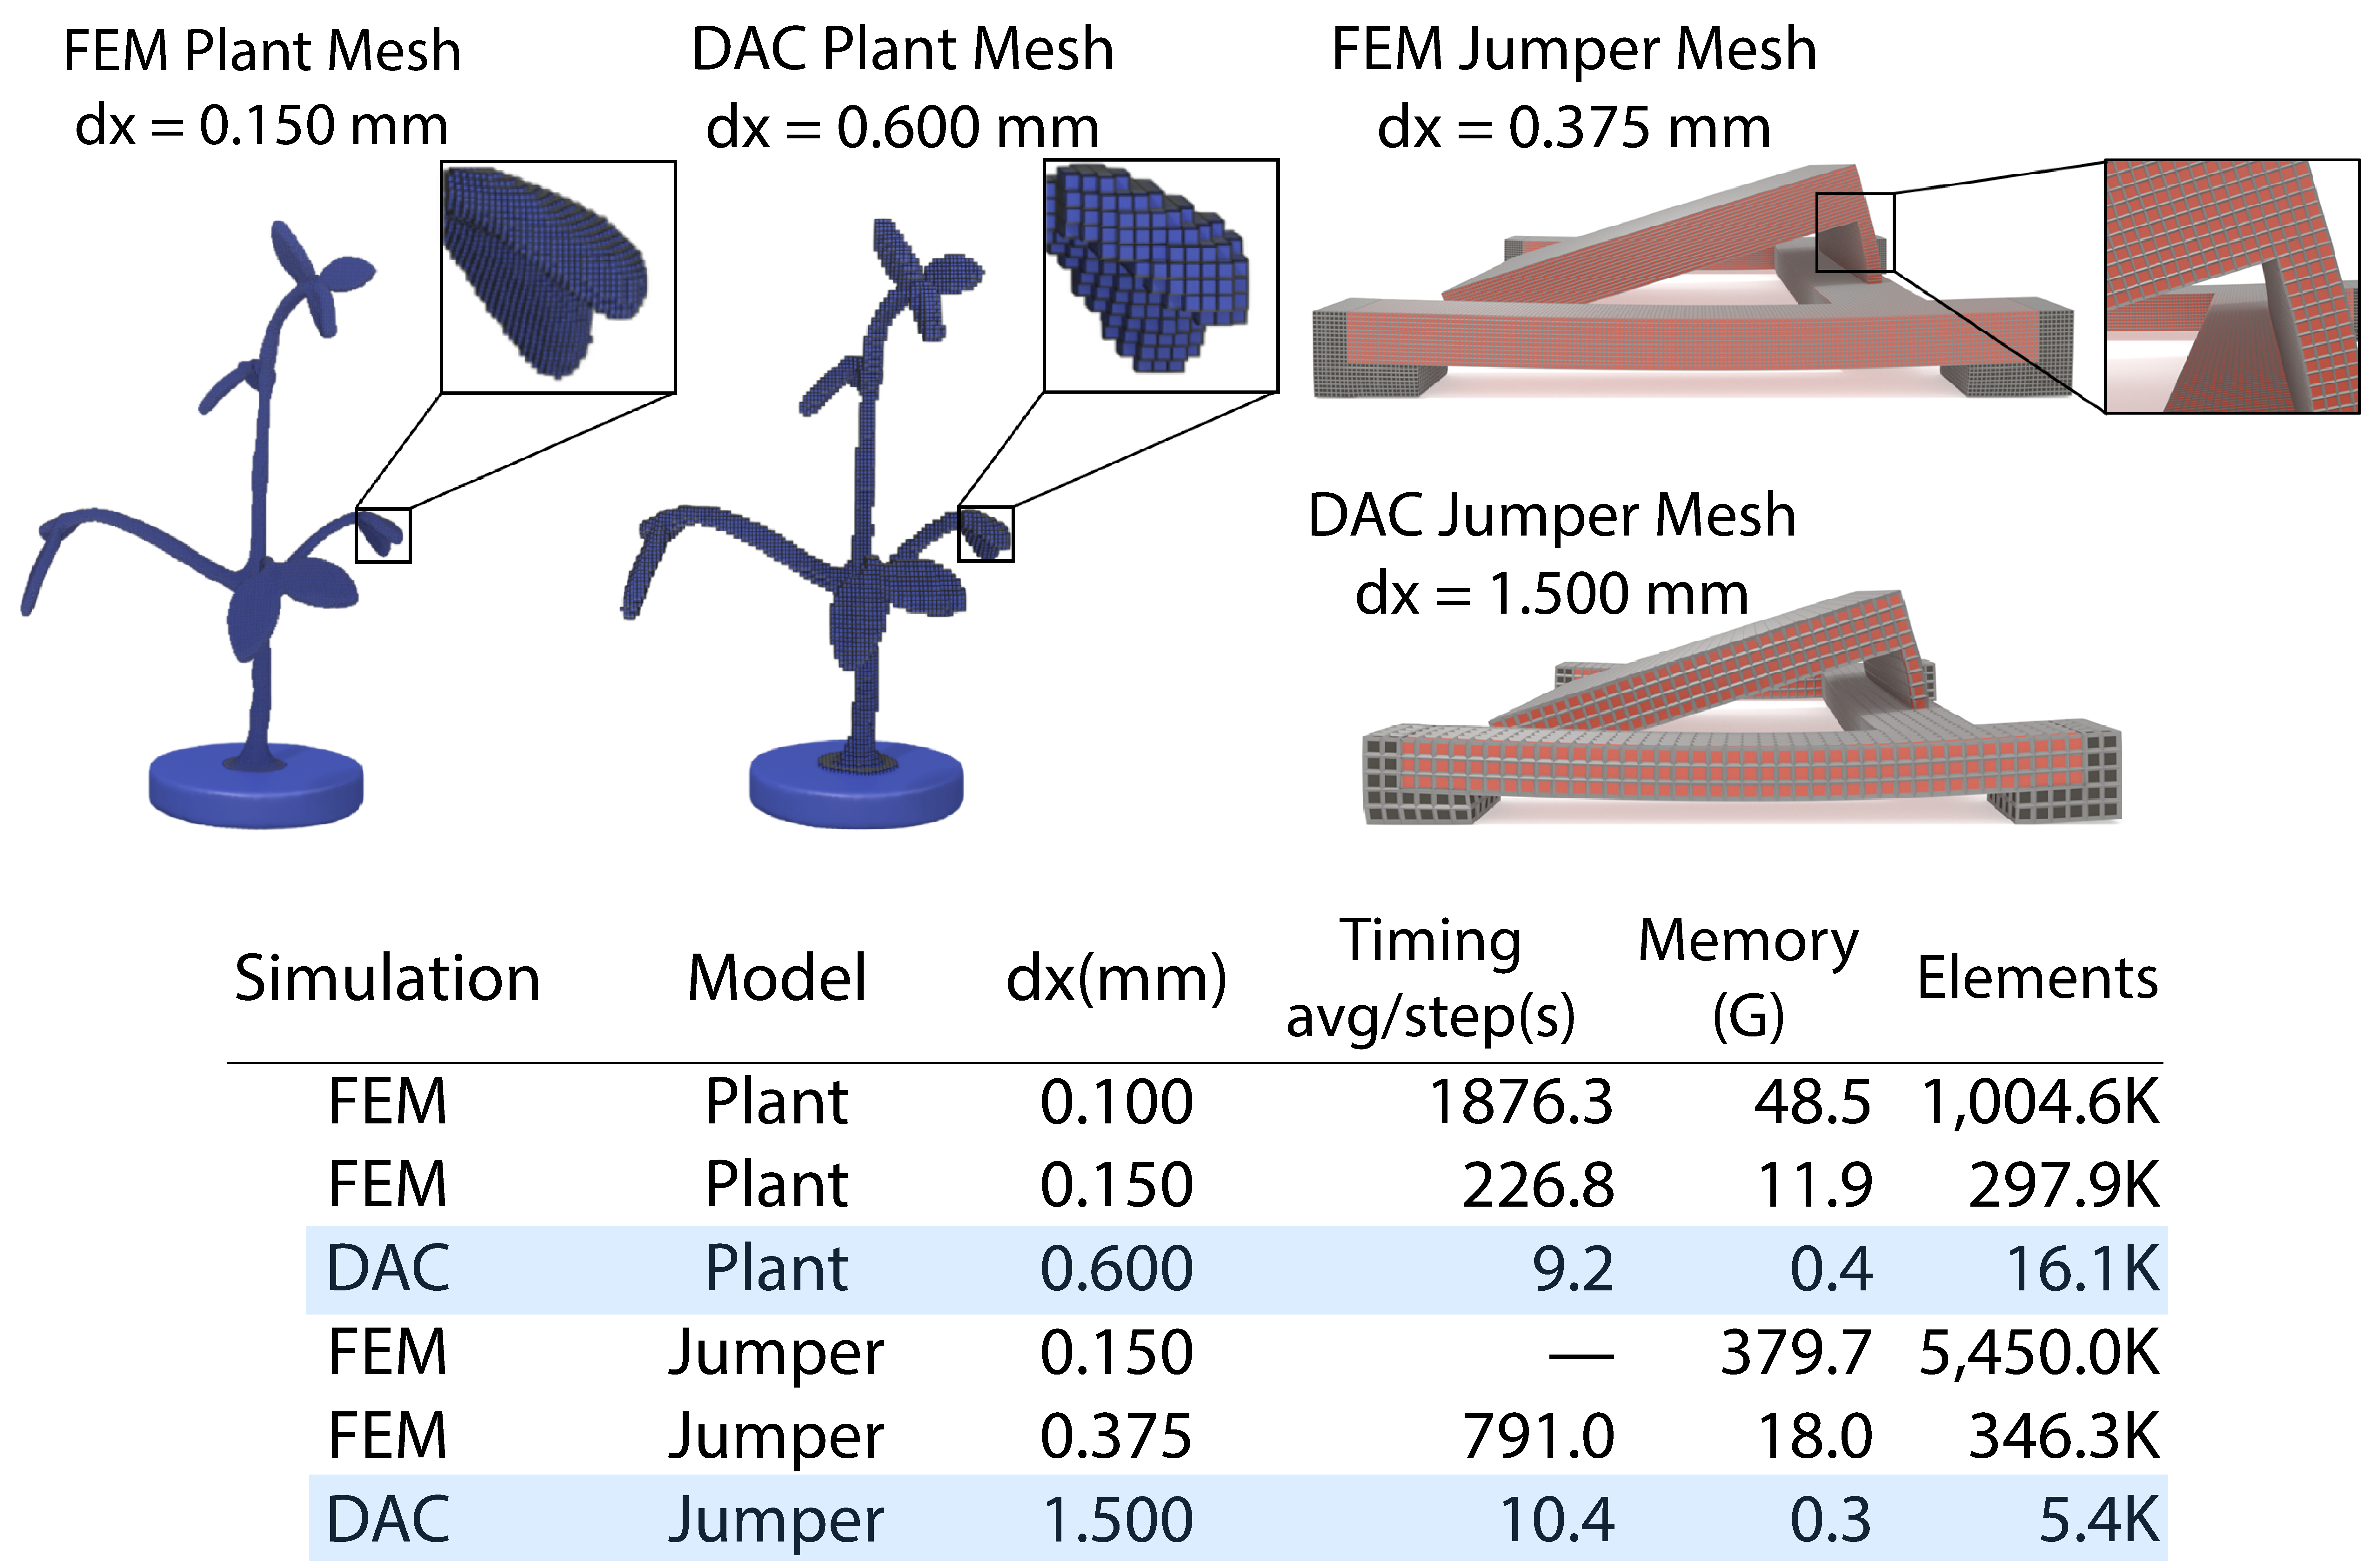
\includegraphics[width=0.8\textwidth]{figs/coarsening_runtime_sim}
	\centering
	\caption{Statistics for our DAC simulations compared with two choices of accurate FE: a convergent FE model, 
		and a validated accurate FE model (validated as matching experimental behavior and modal frequencies are within $5\%$ of convergent values). For each simulation we report the model used (plant and jumper models), the mesh element size,  the average wall-clock time spent per dynamic time step, memory usage, and the number of elements in the simulated mesh. Timings were recorded on an Intel Xeon E5-2666 v3, 2.9Ghz with 4 CPU threads.
	}
	\label{table:suff}
\end{figure}
\section{Boundary Balancing Impact Model}
\label{sec:BBI}

\begin{figure}[h!]
	\centering
	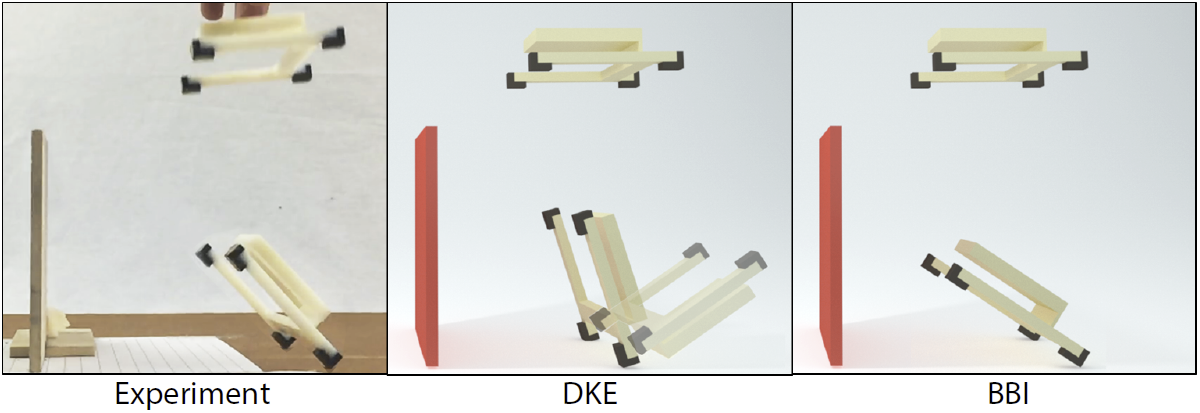
\includegraphics[width=0.8\columnwidth]{images/BBI_jumper_drop.png}
	\caption{Impact model testing with a 3D-printed jumper dropped onto the ground. We show overlaid frames captured, left to right, from an experiment (left) and two corresponding simulations (at $h=10^{-4}s$) that respectively apply DKE (middle) and BBI (right) impact models. In experiment the fabricated jumper lands, bounces up and then rests upright on its feet (left). However, simulation with the DKE model (middle) rebounds too high, flips over and so incorrectly predicts that the jumper will fail by landing on its back after collision (middle). With our BBI model (right), our simulation qualitatively predicts the experimentally determined landing behavior for this design.}
	\label{fig:collision_exp}
\end{figure}

With our DAC discretization in place, we will now derive a new, Boundary-Balancing Impact (BBI) model for FE that gains us accurate prediction of impact-response for the 3D-printed elastic materials we focus on in this work.

\subsection{Complementarity Integration Revisited} 
The nonsmooth Newmark complementarity integrator we reviewed in Section~\ref{sec:simPrelim} has several well-known flaws~\cite{Deuflhard:2008fu} that we illustrate next. In Figure~\ref{fig:BBI_block_compare_all} right, we drop a 3D-printed block from height of 3 cm onto a flat surface. As it is both stiff and highly damped it lands without perceptible rebound. Yet, when we simulate the same drop of the block with the Newmark complementarity integrator the block rebounds up to a height of 0.89 cm; see Figure~\ref{fig:BBI_block_compare_all} left. Errors on this scale are unacceptable in a fabrication design process where they can make the difference between success and failure - see Figure~\ref{fig:collision_exp}.

What is going wrong in these examples? The Newmark discrete velocity update step in (\ref{eq:newmark_free_update}) gives rise to an arbitrary, undesirable (and for elastic materials) generally incorrect choice of restitution. Consider the impact of our material at contact with a normal $\vc n$. Here the complementarity constraints ensure that the new displacement $\delta^{t+1}$ along this normal are zero so that $\vc n^T \delta^{t+1} = 0$. However, although this nicely satisfies position constraints, upon substitution we see that $\vc n^T \vc v^{t+1} =  -\vc n^T \vc v^t$ so that Newmark gives an incorrect, fully elastic (coefficient of restitution $= 1$) effective impact response. Yet the impact response for elastica along an impact boundary should instead be inelastic with the normal velocity on impact along the elastic boundary dissipated completely~\cite{Doyen:2011gka}. In turn this results in much too large rebounds upon impact as we observe in Figures~\ref{fig:collision_exp} and \ref{fig:BBI_block_compare_all}. A related error for complementarity integrators manifests in commonly observed spurious oscillations in positions and tractions along contact boundaries. These oscillations are the combined result of instabilities in contact stresses, velocities and displacements. Notably, both of these issues arise with arbitrary impact geometries, not just in the planar example discussed here.

\subsection{DKE Contact Stabilization} 
To address these widely reported problems,~\citet{Deuflhard:2008fu} introduced a contact stabilization step to filter contact response with projection. They observe that contact forces acting on the material boundary should be balanced and so proposed a now-standard FEM contact-stabilization filter (DKE) that applies an L2-projection that zeroes out normal displacements along the boundary of materials at contact interfaces.  

This projection on displacement is performed at the end of each time step, after the position update (\ref{eq:newmark_contact_implicit}) has been solved. This ensures a correct \emph{inelastic} response at the contact boundary and is effective in producing desirably stabilized contact tractions~\cite{Deuflhard:2008fu,Krause:2012im}. 
Nevertheless, when we compare DKE against experiment (Figures~\ref{fig:collision_exp}, \ref{fig:BBI_block_compare_all}, and \ref{fig:BBI_block_compare_plant}), we see that the DKE projection likewise introduces unacceptably large rebound errors when compared with real-world results.

\begin{figure}
	\centering
	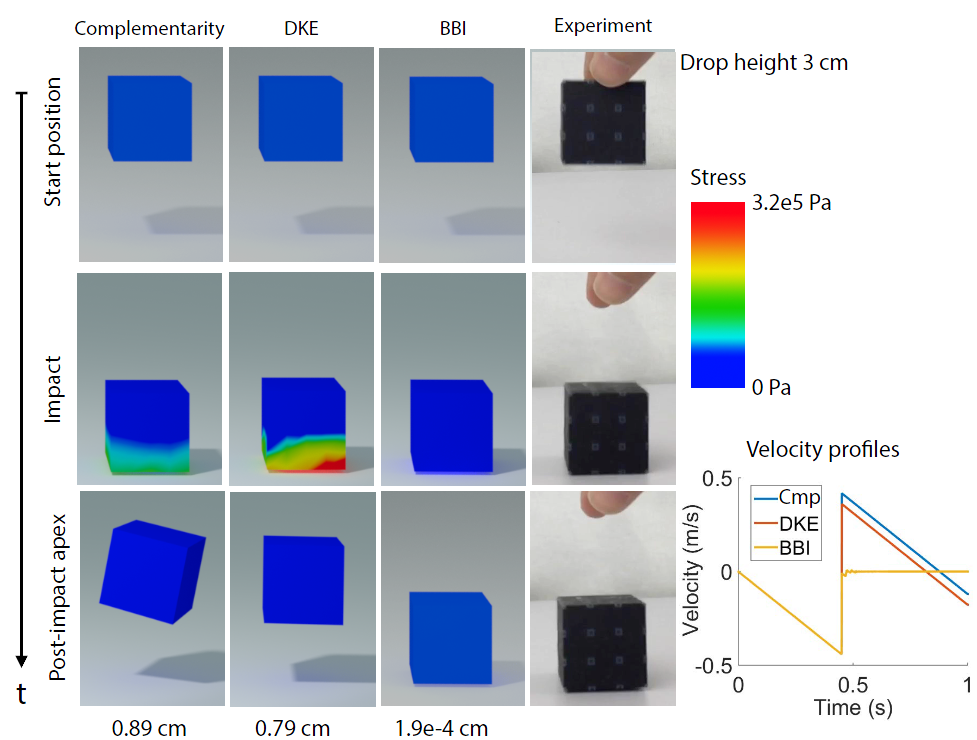
\includegraphics[width=0.8\columnwidth]{images/BBICubeCmp.png}	
	\caption{Impact validation test. A 3D-printed, stiff elastic block is dropped face-first on the ground. Left-to-right we compare the simulated results of three FE impact models  - complementarity, DKE and our BBI model - with experimental results. We show configuration, at start, impact, and post impact maximum rebound height with details on stress distribution at impact, apex height reached, and (inset) the velocity profile for each simulation. As the effective restitution of elastica varies with angle of impact, see below in Figure~\ref{fig:cube_corner} for a comparable oblique drop experiment.}
	\label{fig:BBI_block_compare_all}
\end{figure}

\begin{figure}
	\centering
	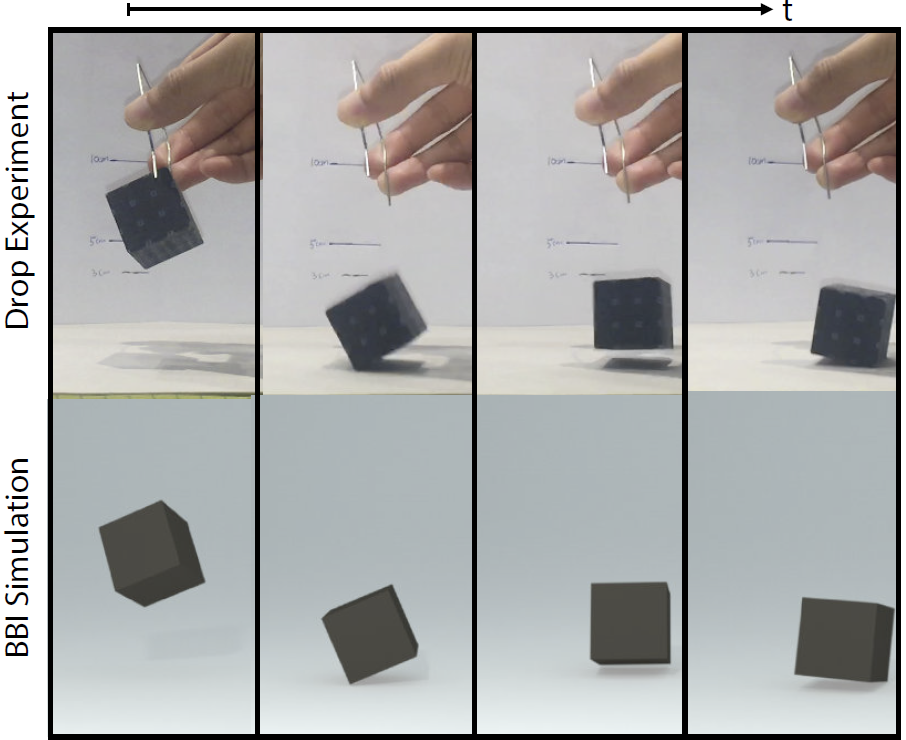
\includegraphics[width=0.6\columnwidth]{images/cubeDropCorner.png}	
	\caption{Comparison of our BBI model to experiment for a 3D-printed cube dropped from an oblique initial orientation.}
	\label{fig:cube_corner}
\end{figure}

\subsection{Boundary Balancing Impact}
To better understand why DKE projection does such a poor job of resolving impacts in our elastic materials, let us consider again our simple dropped block example in Figure~\ref{fig:BBI_block_compare_all}.
We observe that by projecting out just the normal component of displacement along the boundary the DKE method artificially \emph{concentrates} high stresses along the elements just inside the boundary. This can be seen in the impact row of Figure~\ref{fig:BBI_block_compare_all}.
These concentrated stresses effectively load the near-boundary layers which then spring back, introducing a much too large response as seen in the final row of Figure~\ref{fig:BBI_block_compare_all}.
The problem here is that the L2-projection applied is material-oblivious and yet material properties clearly mediate impact response. Compliance distributes contact stresses quickly through an elastic material while, in damped materials, internal friction rapidly attenuates the response. 

With these observations in mind we define a new Boundary Balancing Impact (BBI) model that can effectively impose boundary force-balance in a material-aware fashion. Starting with our base time integrator we define a compliant, discretization- and material-aware metric for projection below. The resulting stabilizing impact model better duplicates results in our design applications and experiments. Upon completing each time step from $t-1$ to $t$ we replace the Newmark update in (\ref{eq:newmark_free_update}) with a compliant boundary projection update
\begin{align}
\begin{split}
\vc c &= 2 \vc \delta^{t+1} - h \vc v^t, \\
\vc A &= \vc M + \frac{h^2}{4} \vc K(\vc q^{t+1}) + \frac{h}{2} \vc D(\vc q^{t+1}) ,\\
\vc d^* &= \argmin_{\vc d} \big\{ \frac{1}{2} \| \vc d - \vc c \|^2_{\vc A} : \vc N^T \vc d \geq 0 \big\},\\
\vc v^{t+1} &= \frac{1}{h} \vc d^*,\\
\vc q^{t+1} &= \vc q^t + \vc \delta^{t+1}.\\
\end{split}
\label{eq:newmark_predictor_proj}
\end{align}

This new impact model projects the explicit predicted velocity displacement, $\vc c$, to the nearest set satisfying force balance on the boundary with respect to the local approximation of both material \emph{stiffness} and \emph{damping}. We find that this effectively distributes the contact-stabilized displacement across the material from the boundary layers. The effect of impact is communicated to the material interior while still ensuring that impacts are correctly inelastic along the active contact boundary.
This leads to accurate predictions of real-world bouncing and rebounds. In our simple drop test we see in the impact row of Figure~\ref{fig:BBI_block_compare_all} that, at impact, response for this damped material has been correctly dissipated and the resulting normal displacement closely matches real world results in the apex row of Figure~\ref{fig:BBI_block_compare_all}. 

As we consider a range of impact angles, as well as impact with more complex geometries, multi-material 3D-prints and self contact we see that BBI still consistently and more accurately captures impact-response behavior. See Figures ~\ref{fig:collision_exp}-\ref{fig:flamingo_contact}. These examples demonstrate the range and complexity of responses obtained by BBI coupling impact to stiff elastic materials with large deformations as well as objects composed of multiple materials undergoing both self-contact and stiction.

\begin{figure}
	\centering
	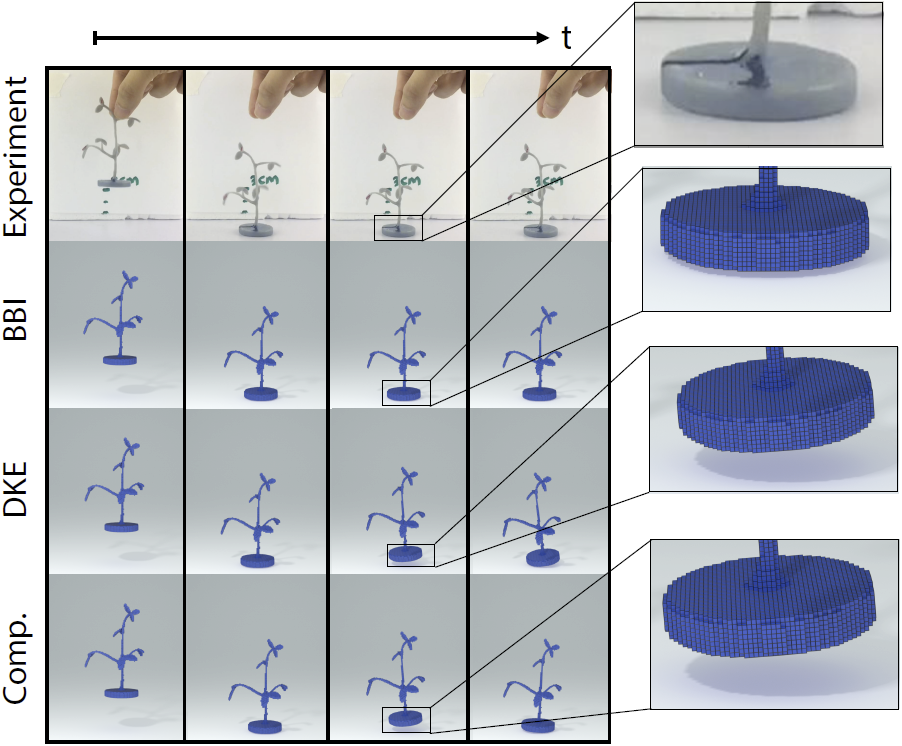
\includegraphics[width=0.8\columnwidth]{images/plantDrop.png}	
	\caption{A drop test of the 3D-printed plant model (digital material). We compare simulated results from Complementarity, DKE and our BBI model with experiment. BBI solely reproduces the observed impact behavior.}
	\label{fig:BBI_block_compare_plant}
\end{figure}

\begin{figure}
	\centering
	\includegraphics[width=\columnwidth]{images/FlamingoDrop.png}	
	\caption{Drop tests of a multi-material 3D-printed flamingo model (Rigur and TangoBlackPlus) from a variety of orientations. While effective restitution of elastica varies with angle of impact, in all cases our BBI simulations agree with experiment.}
	\label{fig:flamingo_contact}
	\vspace{-10px}
\end{figure}
\section{Results and Discussion}
\label{sec:results}

To test our proposed algorithms we compare simulated results generated by DAC and BBI with real-world results experimentally obtained from a range of compliant 3D-printed jumping and throwing mechanisms.
For each mechanism we begin with a dynamic, time-varying goal, e.g., for our \emph{jump-over} goal: ``when pressed and released, jump over a given wall and land upright on the far side'' (see Figure~\ref{fig:over}).

Simulations suitable for fabrication design must accurately predict both when a design fails and when it succeeds, thus we require real world examples of each. Below we outline our approach to creating these mechanism examples for testing, discuss our identification results, and review our implementation. We then detail our experiments comparing DAC and BBI's simulated predictions for each design task below in \S\ref{sec:exp} and validate outcomes of the simulations against repeated user trials in a study discussed in \S\ref{sec:user}.

\subsection{Creating Mechanism Examples} We focus our tests here on jumping-related mechanisms. The analysis and design of jumping mechanisms is an increasingly active~\cite{Anonymous:gFJEnD-w,bergbreiter2007design,Bingham:orient,Bergbreiter:2008te,Jung:2014fh,JeSungKoh:2013ga,Koh:2015cy,Vella:2015cw,ShuguangLi:2015kl}, challenging and practical domain that incorporates high-speed transient dynamics of stiff elastic materials undergoing impact and so is an ideal test case for DAC and BBI.
Research in jumping mechanisms has focused on efficient energy transfer into jump height, see e.g.,~\citet{MinkyunNoh:2012fv}
with aligned research on a range of approaches for controlled jumping~\citep{Loepfe:2015ir,Bartlett:2015he,ShuguangLi:2015kl}. In all cases, to our knowledge, mechanisms have been developed via costly, manual iterations of hands-on experiment, re-design, fabrication and one-off simulations~\citep{Cho:2009jl,Bartlett:2015he}, while even the stable landing of dynamic jumps has remained highly challenging~\citep{Jung:2015gm}.

For each of our jumping and throwing goals (see \S\ref{sec:exp} below) we first attempted to manually create successful designs. We obtained designs that came close to ideal, but, consistent with the above cited literature, we were unable to hand tune these mechanisms to fully satisfy design goals. E.g., for the jump-over goal we found a design that often cleared the wall but did not land upright; see Figure~\ref{fig:over}, left. These mechanisms are our \emph{initial} designs.

Presuming our initial designs are potentially close to successful designs, we perform local optimization over a pair of key design parameters, here generally length and height (see Figure~\ref{fig:params}), to seek a nearby solution. For each mechanism we pose its design goal as an objective and a set of constraints; these functions are detailed in Figure~\ref{table:perf}. To evaluate these objectives and constraints we apply DAC and BBI simulation at each design sample queried by the optimizer. Statistics for the numbers of simulation samples, iterations and timings for performing these local optimizations are summarized in Figure~\ref{table:perf}.

For all these examples we found that a relatively small number of iterations were needed to find successful designs;  this suggests that our initial, hand-tuned designs are close to solutions in a basin. However, practical design optimization would demand a global optimization strategy to resolve non-convexity. In such general cases initial designs can be expected to start far from optima while the search space is often large - local optimization would be insufficient.

The mechanisms found by this process are our \emph{final} designs. We compare the trajectories and outcomes predicted by BBI and DAC against the real world initial and final mechanisms: validation results are detailed for each example below in \S\ref{sec:exp}, while our user study results are presented in \S\ref{sec:user}. The uncut video footage of all experiments are available online~\cite{Video}.

\begin{figure}[h]
	\centering
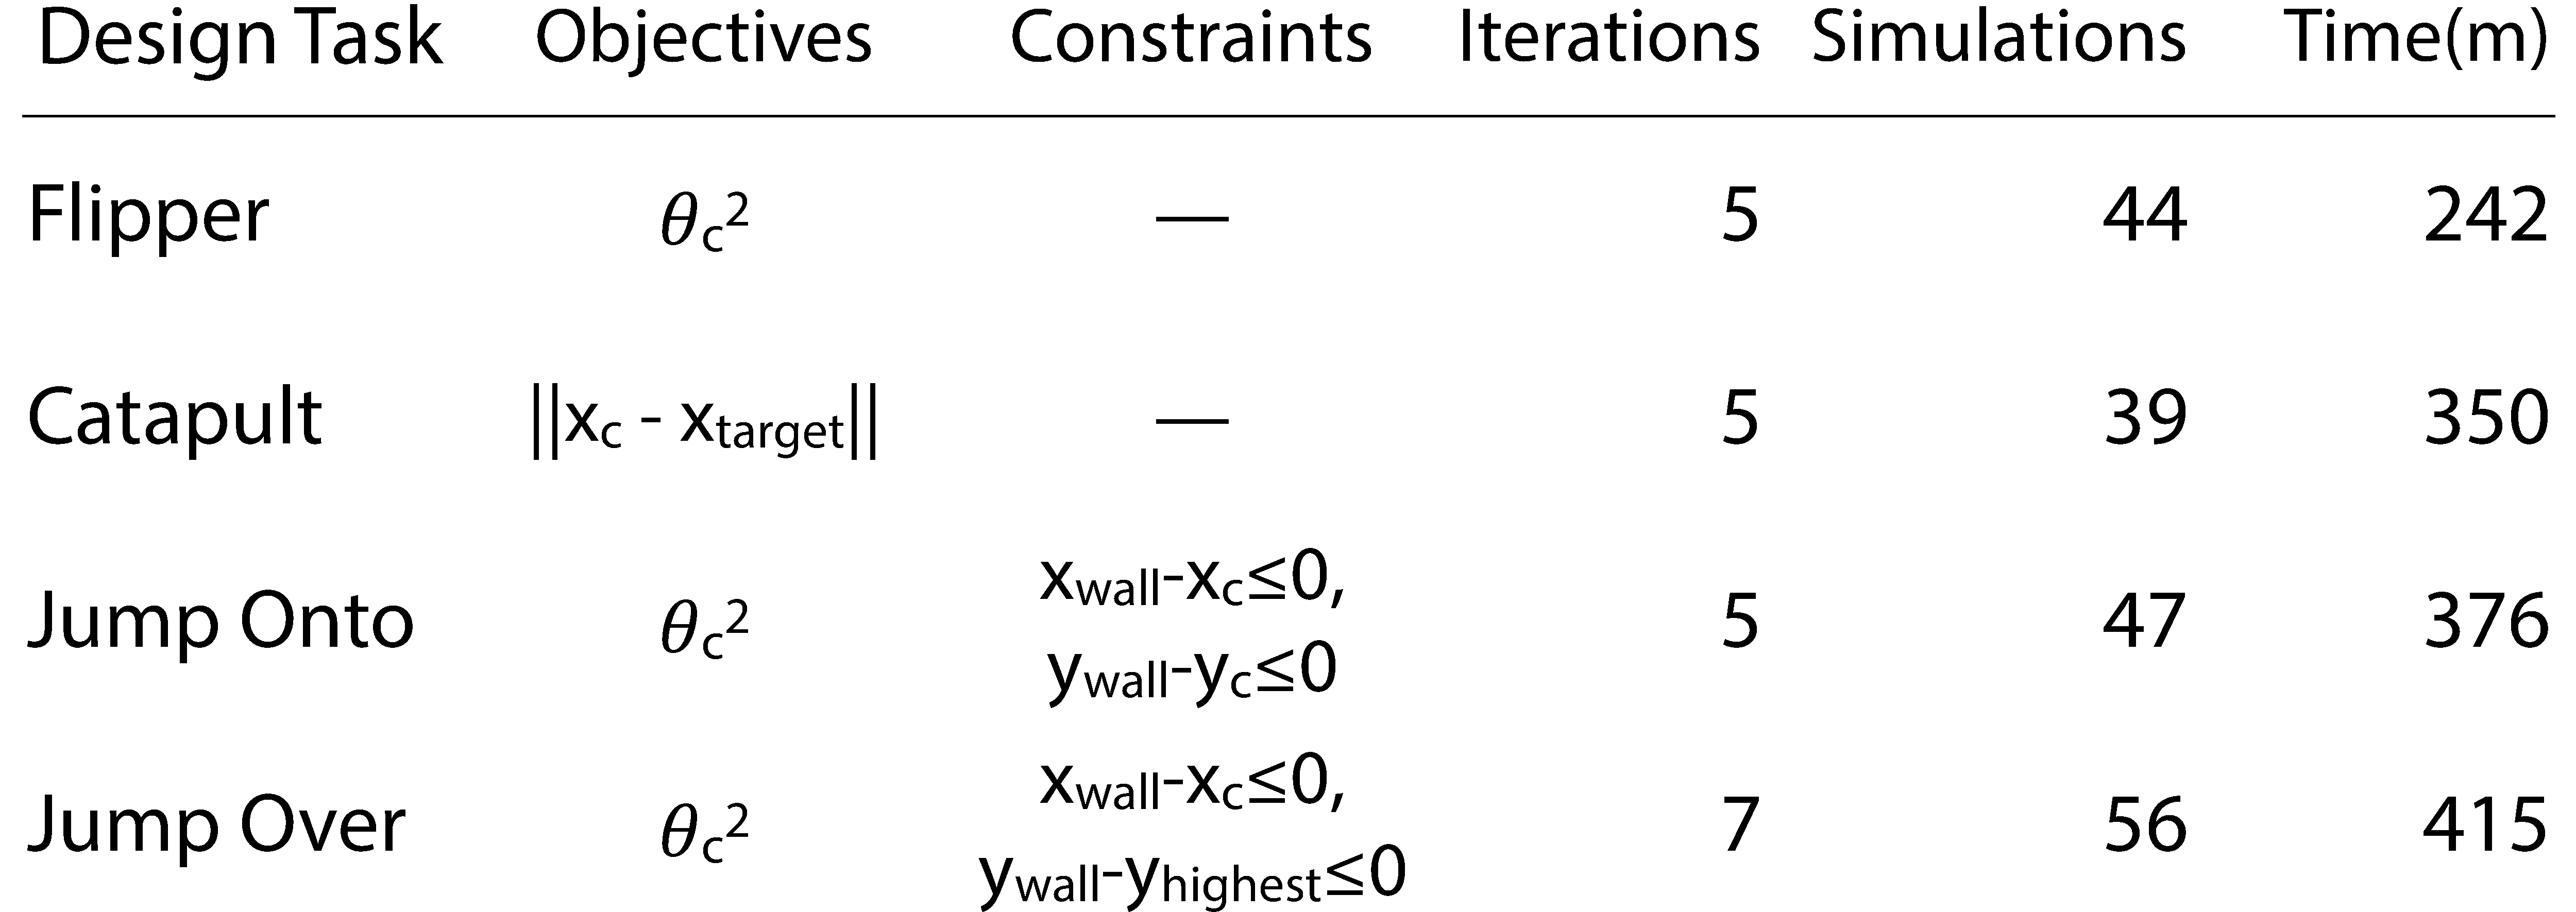
\includegraphics[width=0.7\columnwidth]{figs/optTable.pdf}
\caption{Design optimization statistics. For each dynamic design optimization we report the design task objectives and constraints applied, the number of optimization iterations performed, the total number of simulations performed for each design and finally the total wall-clock time (minutes) spent in design optimization. Sampled frames for each simulated and corresponding fabricated mechanism designs are given in Figures~\ref{fig:flipper}--\ref{fig:more_flippers} and design parameters optimized over are summarized in Figure~\ref{fig:params}. Here $\theta_c$ and $\vc{x}_c$ represent jumper angle of rotation and catapult projectile center-of-mass position at landing while $\vc{x}_{\text{target}}$ is the desired projectile target.
}
\label{table:perf}	
\end{figure}

\begin{figure}[h!]
\centering
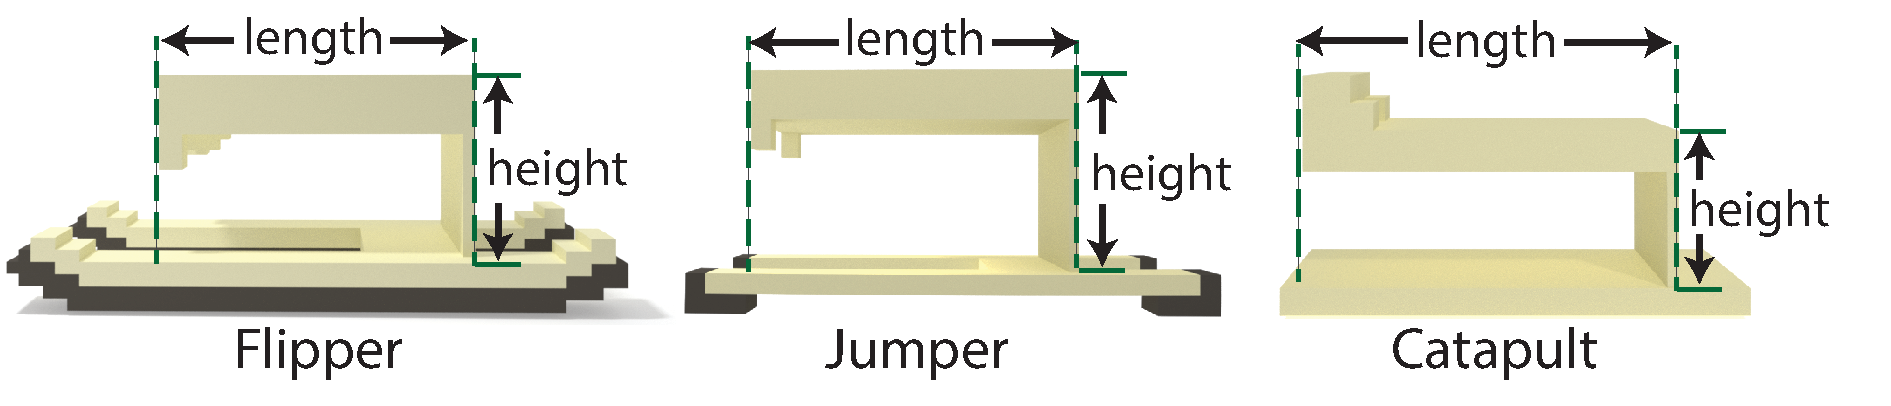
\includegraphics[width=0.7\textwidth]{figs/param.pdf}
\caption{Design geometries and parameters.}
\label{fig:params}
\end{figure}	

\subsection{Implementation}

All results are computed on an Amazon EC2 compute-optimized instance with 4 CPU threads (Intel Xeon E5-2666 v3, 2.9Ghz), while all mechanisms were printed on a Objet500.
While DAC and BBI give us orders of magnitude speedups for predictive simulation of deforming dynamics, our experiments (see Supplemental) show that dynamic FE simulation is unnecessary when modeling initial loading as well as during some portions of free-flight. With careful book-keeping and mapping of state simpler and more efficient models can be employed during these phases to gain further speedup.
When initially loading mechanisms, e.g., when pressing down a jumper in Figure~\ref{fig:simulationStage}, we observe that the process is effectively quasistatic and so simulate with an efficient quasistatic solver detailed in our Supplemental. Upon completion of the initial loading we map state to our full dynamic solver with DAC and BBI.
We also track the time-varying elastic potential energy stored in simulated compliant objects. When damping causes this internal potential to fall to zero, e.g., during portions of free-flight, we switch from our full DAC discretization to a rigid body discretization. We use DMV~\cite{Moser:1991dl}, an efficient energy--momentum preserving rigid-body integrator, to then time step the system in SE(3) coordinates until the next collision is reached, at which point we map rigid-body state back to the DAC model to capture the new deformation dynamics at impact. See our Supplemental for details on this process.

\subsection{Identification}

\begin{figure}[h!]
\centering
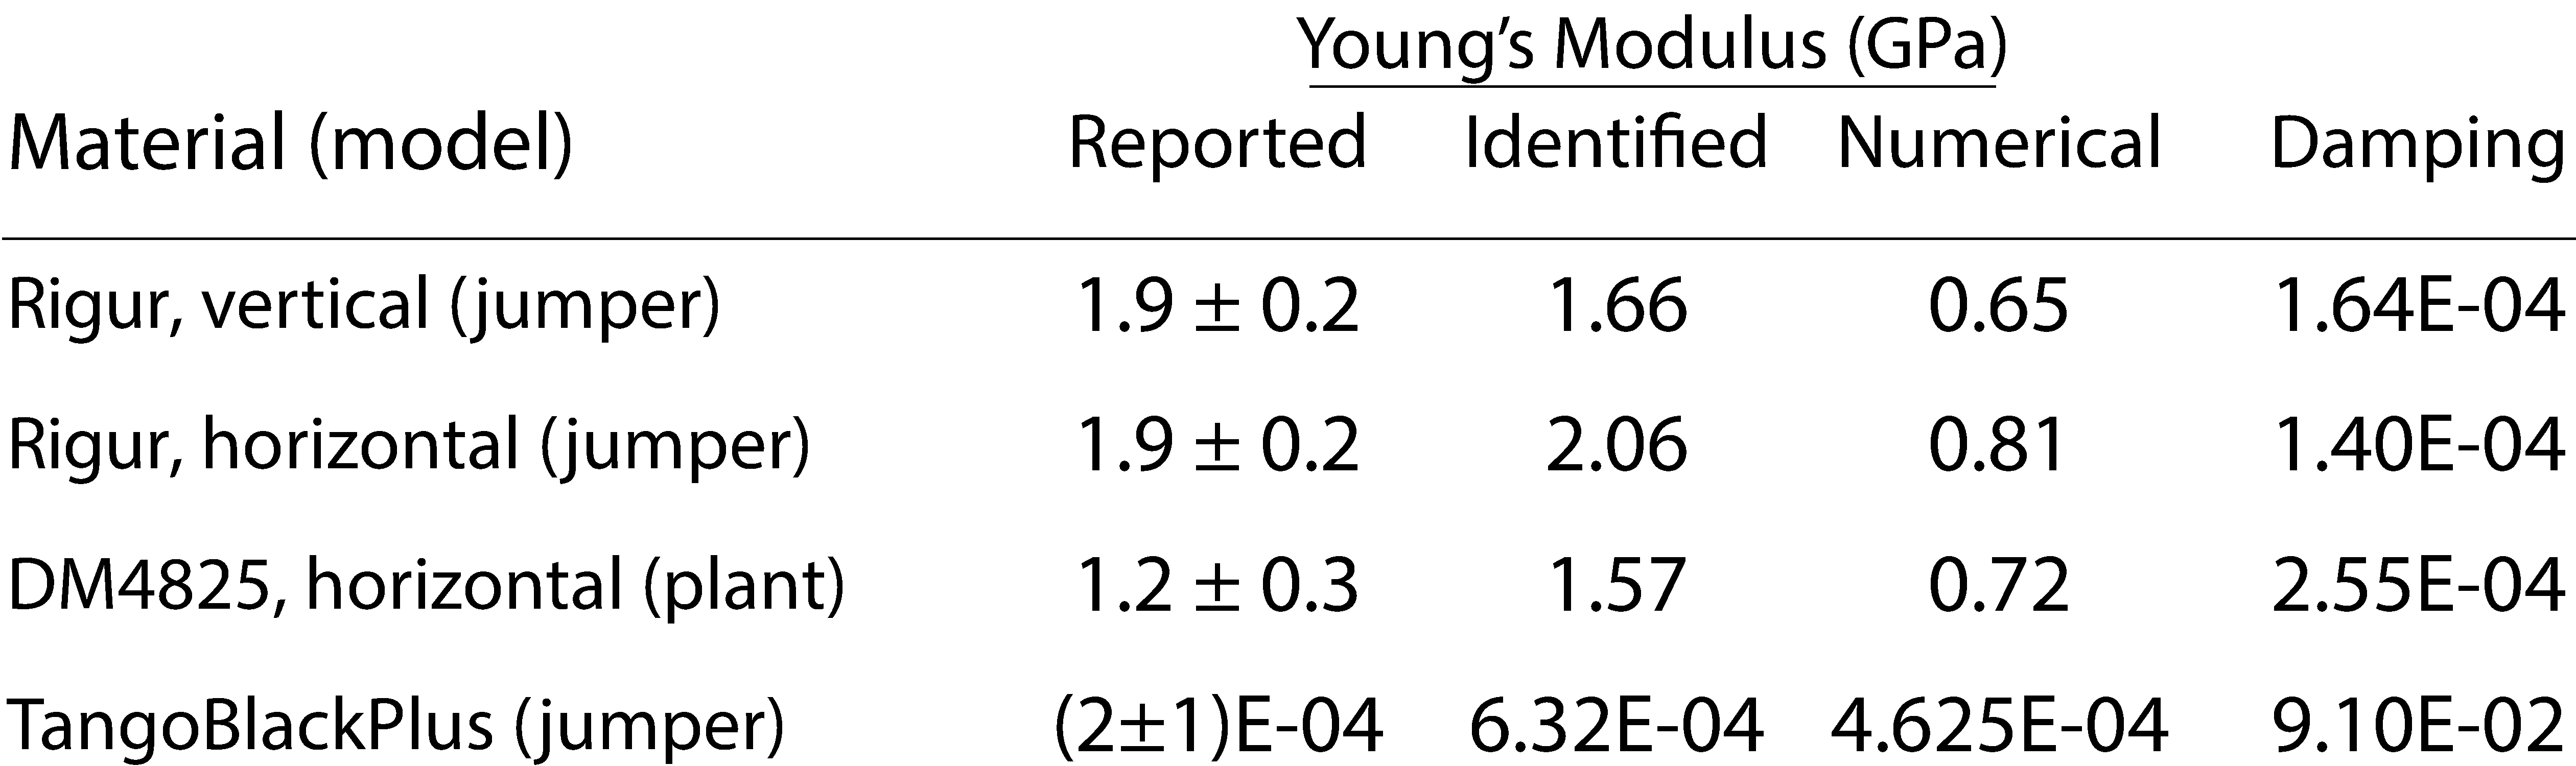
\includegraphics[width=0.45\textwidth]{figs/materials_table}
\caption{Material parameters identified by our fine and coarse matching against calibration. Left to right we list previously reported Young's moduli for vertically and horizontally oriented prints compared with our identified moduli. We then report the matched numerical moduli we use for each for our DAC models and finally, list previously unreported damping parameters we identify and use in our simulations. 
}
\label{fig:identified_params}
\end{figure}

We compute each DAC model's coarse mesh resolution and material parameters using the measurement procedure described above in \S\ref{sec:DAC}; see also Figure~\ref{fig:vibration_match}. We model heterogeneous materials by computing numerical Young's moduli for soft (TangoBlackPlus) and rigid (Rigur RGD450) materials and coarsening as much as possible while retaining a single material per element. A major benefit of our coarsening scheme is that it identifies both actual and numerical moduli and damping parameters of real-world materials. Figure \ref{fig:identified_params} details these parameters. The damping parameters we present here have not, to our knowledge, been previously identified in the literature. On the other hand, in our experiments and simulations we find that the previously identified Poisson's ratio for our printed materials~\cite{major2011}, at $0.45$, is effective, and keep it fixed at this value for all examples reported here.

\begin{figure}
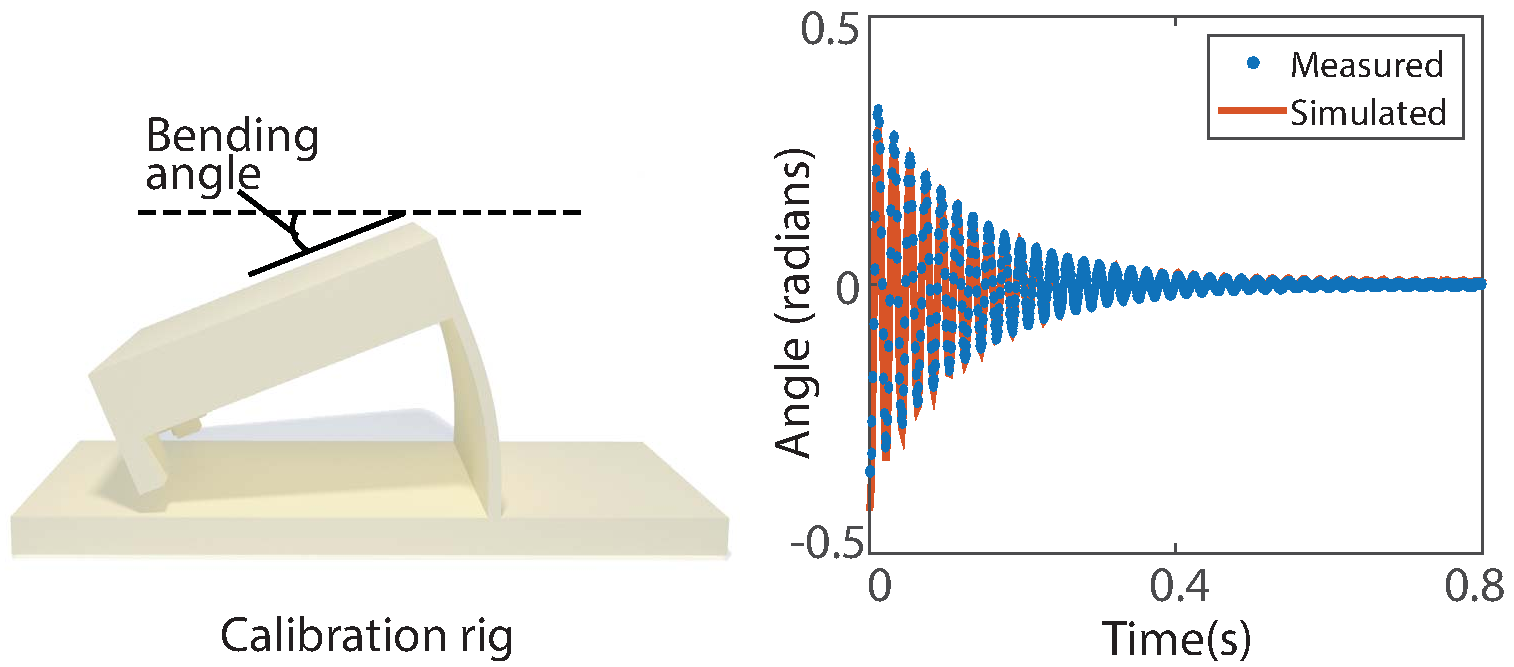
\includegraphics[width=0.45\textwidth]{figs/measure.pdf}
\caption{Measured and simulated vibrations of a 3D-printed jumper (Rigur) model (magnify the plot for details of fit).}
\label{fig:vibration_match}
\end{figure}

\subsection{Experiments}
\label{sec:exp}

\changed{In this section we detail the individual design examples. We visually compare the trajectory behavior of both the real world fabricated initial and final mechanisms with corresponding DAC and BBI simulation results at the same parameters. In the following section we then discuss the results of the user study we perform to evaluate the results of initial and final fabricated mechanisms over repeated user trials comparing against DAC and BBI predicted simulation outcomes.}

\begin{figure}[h!]
\includegraphics[width=\columnwidth]{./figs/ResultsFlipper.pdf}
\caption{A comparison of experimental (bottom) and DAC/BBI simulated (top) results for initial (left) and final (right) designs of a flipping mechanism.}
\label{fig:flipper}	
\end{figure}

\paragraph{Flipper}
Our first design example is a simple forward flipping jumper. We begin with the geometry in Figure~\ref{fig:flipper} left, load the jumping model by pressing down and then releasing. The design goal is a shape that, upon release, jumps forward into the air, flips and then lands stably on its feet, see e.g., Figure~\ref{fig:simulationStage}. 
See Figure~\ref{fig:flipper} comparing simulated and experimental trajectories for both initial and final design samples.

\begin{figure}[h!]
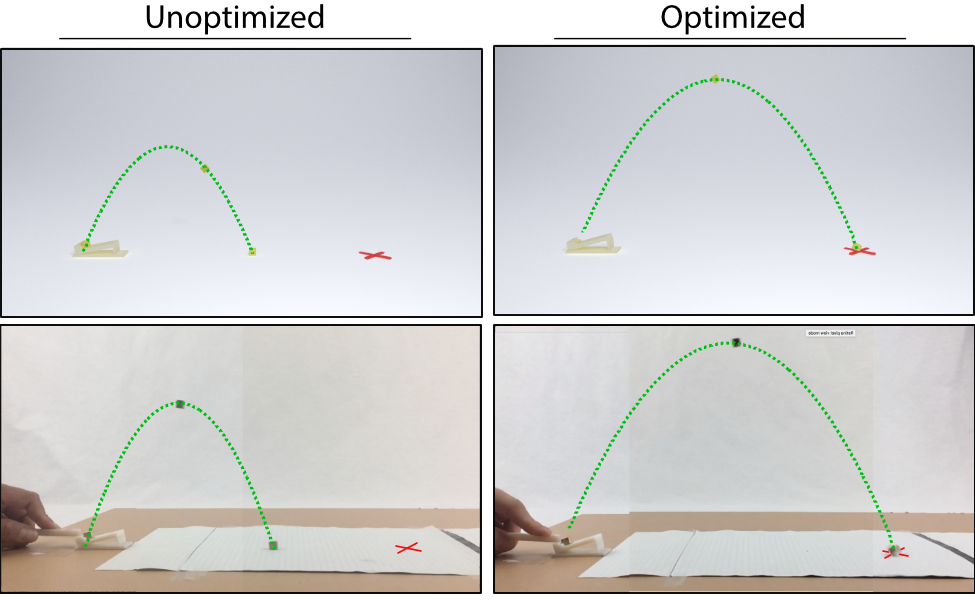
\includegraphics[width=\columnwidth]{./figs/ResultsCatapult.pdf}
\caption{A comparison of experimental (bottom) and DAC/BBI simulated (top) results for initial (left) and final (right) designs of the catapult mechanism.}
\label{fig:catapult}	
\end{figure}

\paragraph{Catapult}
Our next design example is a catapult mechanism. By adding a firing basket to the above flipper geometry, fixing the mechanism base to the ground, and then adding a projectile cube in the basket to the design model we obtain a catapult for throwing metal cubes at targets. This system requires modeling the sliding contact and impact between the cube and basket. The design goal here is to find a catapult geometry that, under loading produces the correct combination of launch position and release velocity for the catapult arm and block so that the block hits a predetermined target. 
See Figure~\ref{fig:catapult} comparing simulated and experimental trajectories for both initial and final design samples.

\begin{figure}[h!]
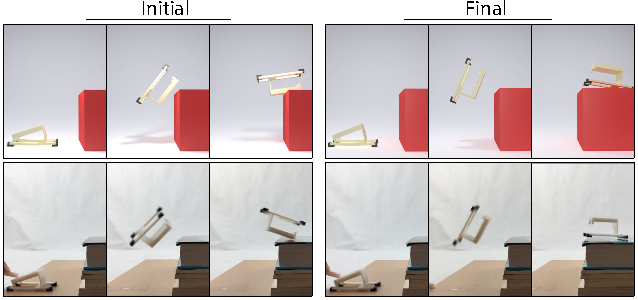
\includegraphics[width=\columnwidth]{./figs/ResultsOnto.pdf}
\caption{A comparison of experimental (bottom) and DAC/BBI simulated (top) results for initial (left) and final (right) designs for a jumper mechanism to jump onto a platform and land upright.}
\label{fig:onto}	
\end{figure}

\paragraph{Jumping onto obstacles}
Here we consider a design example where the goal is  
to find a geometry for a 3D-printed jumper mechanism that, upon release, jumps forward and upwards into the air, flips (possibly multiple times) and then lands stably upon its feet on top of a flat obstacle, see e.g., Figure~\ref{fig:onto}. 
See Figure~\ref{fig:onto} comparing simulated and experimental trajectories for both initial and final design samples.

\begin{figure}[h!]
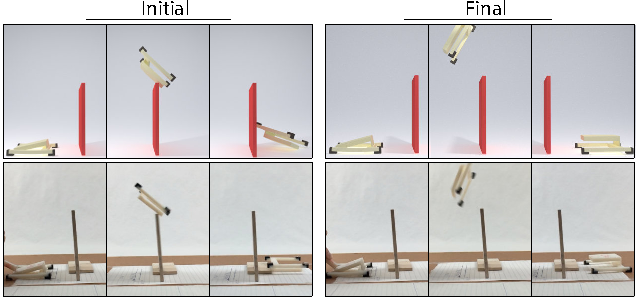
\includegraphics[width=\columnwidth]{./figs/ResultsOver.pdf}
\caption{A comparison of experimental (bottom) and DAC/BBI simulated (top) results for initial (left) and final (right) designs for a jumper mechanism to jump over a wall of specified height and land upright.}
\label{fig:over}	
\end{figure}

\paragraph{Jumping over obstacles}
In this example, the goal is to find a geometry for a 3D-printed mechanism that, upon release, jumps forward and upwards high enough into the air to clear a wall, flip (possibly multiple times) over it and then land stably on the other side. 
See Figure~\ref{fig:over} comparing simulated and experimental trajectories for both initial and final design samples.

\begin{figure}[h!]
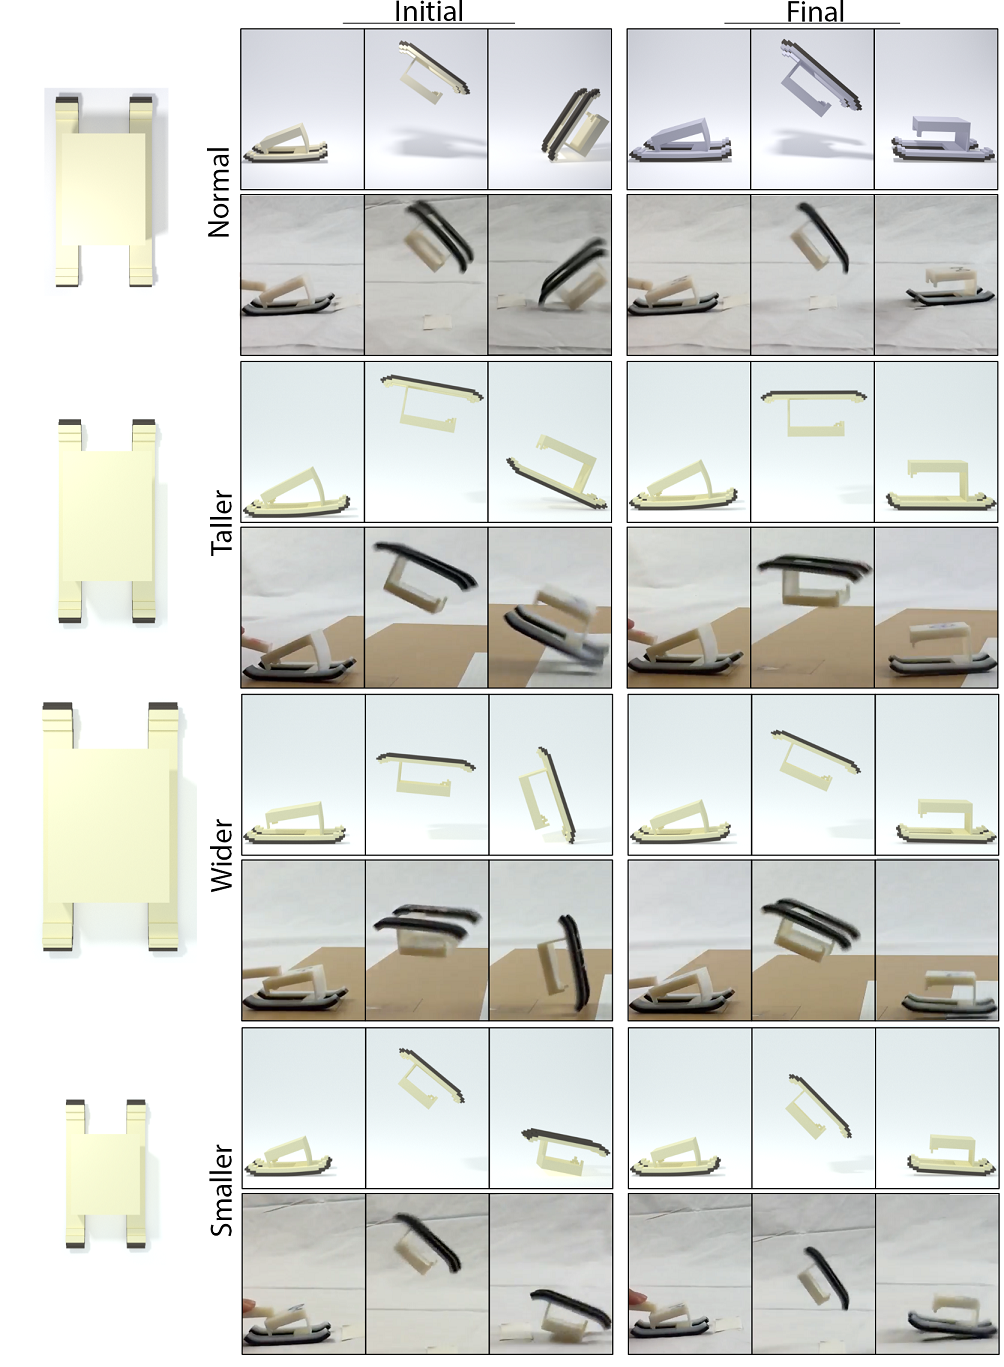
\includegraphics[width=\columnwidth]{./figs/ResultsAllFlippers}
\caption{\changed{A comparison of experimental (bottom) and DAC/BBI simulated (top) results for six more design samples: initial (left) and final (right) designs of variations on the flipping mechanism (``Normal'').}}
\label{fig:more_flippers}	
\end{figure}

\paragraph{Flipper variations}
We additionally evaluate six further design example comparisons between fabricated mechanisms and DAC and BBI simulated trajectories over a range of flipper mechanism variations. In Figure~\ref{fig:more_flippers} we compare initial and final designs created by three variations away form the base initial (``normal'') flipper mechanism design.

\subsection{User Study Results}
\label{sec:user}
Here we present the results of a user study evaluating the goal outcomes of initial and final fabricated mechanisms over repeated user trials as compared against outcomes predicted by DAC and BBI.

\begin{figure}[h!]
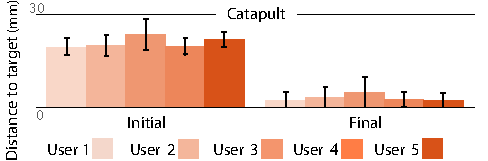
\includegraphics[width=\columnwidth]{./figs/UserStudyCatapult.pdf}
\caption{Statistics summarizing our user study comparing results from trials with our initial and final \emph{catapult} mechanisms. We report the distance to target per trial. The final catapult design dramatically outperforms its initial counterpart, consistently, across all users, coming close to matching DAC/BBI predicted outcomes.}
\label{fig:userStudyCatapult}
\end{figure}

\begin{figure*}[hpt!]
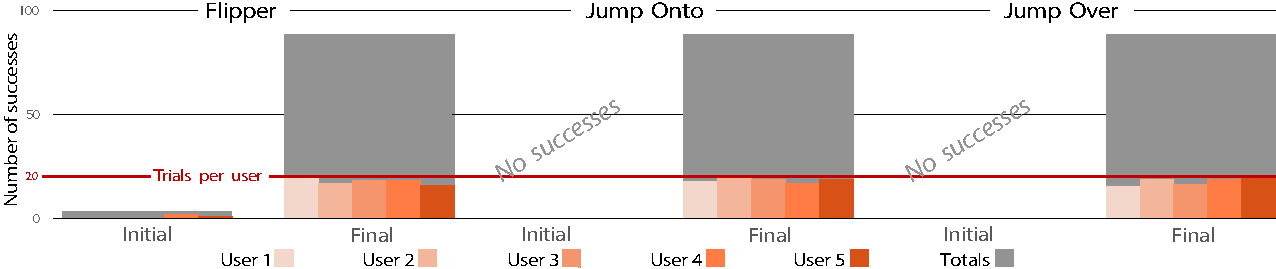
\includegraphics[width=\textwidth]{./figs/UserStudyJumpers.pdf}
\caption{
Statistics summarizing our user studies comparing results from trials (left to right) with our our initial and final  \emph{flipper}, \emph{jump-onto}, and \emph{jump-over} mechanisms. In orange bars we report the number of successes per user, while in grey we report total successes per mechanism across all trials. Note that  initial designs for both the \emph{jump-onto} and \emph{jump-over} have no successes at all, while, across all three mechanisms, final designs dramatically outperform their initial counterparts. This success is consistent across all users - closely matching DAC/BBI predicted outcomes.}
\label{fig:userStudyJumpers}
\end{figure*}

We asked five users to perform twenty attempts each with both the initial and final versions of each of the above mechanisms; the flipper, catapult, jump onto and jump over. For the flipper, jump onto and jump over mechanisms we count the number of successful attempts for each user; see Figure~\ref{fig:userStudyJumpers}. Here we define goal success as satisfying the objectives and constraints posed by each design as described above; e.g. flipping, clearing all obstacles, and landing feet down on the desired area (Figures \ref{fig:flipper}, \ref{fig:onto} and \ref{fig:over}).
In Figure~\ref{fig:userStudyJumpers} we summarize the total number of successes for each user per optimized and unoptimized design as well as the aggregate totals. For the optimized and unoptimized catapult designs we report the mean distance to the target in millimeters and the standard deviation for each user~(\autoref{fig:userStudyCatapult}). 

In order to consistently apply the loading force to each mechanism, users are instructed to fully load each mechanisms by pressing the top until it makes contact with the bottom. We ask users to apply the loading force with a 3D printed bar at a designated loading point marked on each mechanism with permanent marker. The user then deformed the mechanism to the loaded state and released the load with a sliding motion, similar to the launching motion in Tiddlywinks. This ensures that contact break between the stick and the mechanism is close-to instantaneous and consistent.  The same criteria are used in simulation to obtain comparable loading. The Objet500 we employ in all our fabrication examples works at 85 microns precision while our design parameter changes are on the order of millimeters and are thus be reliably manufactured. Additionally to further  minimize variability in experimental conditions we use the same printer for all examples and always print in the top left area of the build tray. We orient models consistently and perform experiments within two weeks of printing to avoid long-term material degradation - an interesting topic for future modeling and design research.

Throughout the study, mechanism goal outcomes consistently matched those predicted by their corresponding DAC/BBI simulations. Final, optimized, mechanisms were much more reliable than their initial counterparts - under simulation these were successful. In terms of jumping (flipping, over, onto) tasks final designs completed more than $85\%$ of their attempts for every task - close to matching DAC/BBI predicted success. while the initial designs successfully completed the simplest flipping task in $3\%$ of all attempts~(\autoref{fig:userStudyJumpers}) and had zero successes for the jump-onto and jump-over tasks - matching DAC/BBI predicted failure. This large difference validates that designed mechanism successes are quite reliably modeled by DAC/BBI.
For instance, our catapult design achieves a $10\times$ reduction in mean error with respect to target distance for all users. Note that here there is a small increase in standard deviation due to the fact that our optimized design of the catapult necessarily throws the cube much further, amplifying any variation errors in initial targeting~(\autoref{fig:userStudyCatapult}).
For supporting evidence of each mechanism's experimental behavior please see our supplemental materials which include uncut videos~\cite{Video} of all user studies.